% -*- coding: UTF-8 -*-
% hello.tex

\documentclass[UTF8,oneside]{ctexbook}

% \usepackage{xeCJK}
\usepackage[utf8]{inputenc}

% load paralist before enumitem
\usepackage{paralist}

\usepackage{hyperref}
\hypersetup{pdftex,colorlinks=true,allcolors=blue}
\usepackage{hypcap}

\usepackage{color}
\usepackage[usenames, dvipsnames, svgnames, table]{xcolor}
% \pagecolor{gray}

\usepackage{makeidx}
\makeindex

\usepackage{amsmath}
\usepackage{mathtools}

\usepackage{listings}
\usepackage{multicol}
\usepackage{fancybox}
\usepackage{tcolorbox}
\usepackage{enumitem}

\usepackage{indentfirst}

\newenvironment{enumbox}[0]{
    \begin{tcolorbox}
    \begin{compactenum}
} {
    \end{compactenum}
    \end{tcolorbox}
}

\newenvironment{itembox}[0]{
    \begin{tcolorbox}
    \begin{compactitem}
} {
    \end{compactitem}
    \end{tcolorbox}
}

% table
\setlength{\arrayrulewidth}{1pt}
\setlength{\tabcolsep}{16pt}
\renewcommand{\arraystretch}{2.5}
\newcolumntype{s}{>{\columncolor[HTML]{AAACED}} p{3cm}}

\arrayrulecolor[HTML]{DB5800}

\usepackage{tikz,mathpazo}
\usetikzlibrary{positioning, fit, matrix, shapes, arrows, chains, trees, arrows.meta}

% \bibliographystyle{plain}
% \bibliography{math}

\tikzset{%
  >={Latex[width=2mm,length=2mm]},
  % Specifications for style of nodes:
            base/.style = {rectangle, rounded corners, draw=black,
                           minimum width=4cm, minimum height=1cm,
                           text centered, font=\sffamily},
  activityStarts/.style = {base, fill=blue!30},
       startstop/.style = {base, fill=red!30},
    activityRuns/.style = {base, fill=green!30},
         process/.style = {base, minimum width=2.5cm, fill=orange!15,
                           font=\ttfamily},
}

% 摘录
\usepackage{verbatim}
\usepackage{libertine}
\usepackage{graphicx}
\usepackage{framed}

\newcommand*\openquote{\makebox(25,-22){\scalebox{5}{``}}}
\newcommand*\closequote{\makebox(25,-22){\scalebox{5}{''}}}
\colorlet{shadecolor}{Azure}

\makeatletter
\newif\if@right
\def\shadequote{\@righttrue\shadequote@i}
\def\shadequote@i{\begin{snugshade}\begin{quote}\openquote}
\def\endshadequote{%
\if@right\hfill\fi\closequote\end{quote}\end{snugshade}}
\@namedef{shadequote*}{\@rightfalse\shadequote@i}
\@namedef{endshadequote*}{\endshadequote}
\makeatother

\usepackage[normalem]{ulem}

\newcommand{\hl}{\bgroup\markoverwith
  {\textcolor{yellow}{\rule[-.5ex]{2pt}{2.5ex}}}\ULon}

%\usepackage{soul}

%\newcommand{\hlc}[2][yellow]{{%
%    \colorlet{foo}{#1}%
%    \sethlcolor{foo}\hl{#2}}%
%}

% todonode
\usepackage{lipsum}                     % Dummytext
\usepackage{xargs}                      % Use more than one optional parameter in a new commands
% 
\usepackage[colorinlistoftodos,prependcaption,textsize=tiny]{todonotes}
\newcommandx{\unsure}[2][1=]{\todo[linecolor=red,backgroundcolor=red!25,bordercolor=red,#1]{#2}}
\newcommandx{\change}[2][1=]{\todo[linecolor=blue,backgroundcolor=blue!25,bordercolor=blue,#1]{#2}}
\newcommandx{\info}[2][1=]{\todo[linecolor=OliveGreen,backgroundcolor=OliveGreen!25,bordercolor=OliveGreen,#1]{#2}}
\newcommandx{\improvement}[2][1=]{\todo[linecolor=Plum,backgroundcolor=Plum!25,bordercolor=Plum,#1]{#2}}
\newcommandx{\thiswillnotshow}[2][1=]{\todo[disable,#1]{#2}}
%

\usepackage[simplified]{pgf-umlcd}

\title{LICH架构文档}
\author{董冠军}
\date{\today}

\begin{document}

\maketitle
\tableofcontents

\listoftodos[Notes]

\part{项目管理}

\chapter{移动集采}

产品评估:功能和质量。质量包括:可靠性,性能,QoS,可扩展性(负载均衡),用户体验(管控,交互,接口)等方面。

性能不是一个值,而是不同场景下的特征曲线。性能是系统配置和负载的函数:$P=F(S, W)$。
精简配置,快照,故障,实现机制等因素都会影响性能及其抖动。

\section{CheckList}

对标\hl{移动集采测试规范}

\subsection{Hardware}

同质化项:
\begin{enumbox}
\item 开机Logo
\item 贴标
\item 开机卡,需断电源
\end{enumbox}

\subsection{Software}

标前测试:
\begin{enumbox}
\item 管理系统相关Logo
\item 上架
\item 安装
\item 性能测试
\end{enumbox}

BUG
\begin{enumbox}
\item etcd依赖于物理时间
\item bcache拔cache盘后需要重启服务器
\end{enumbox}

性能:
\begin{enumbox}
\item \hl{打开chunk parallel开关}
\item \hl{禁用core}
\item 优化Log
\item O3编译
\item -g
\item 代码段
\end{enumbox}

功能:
\begin{enumbox}
\item IPv6
\item SNMP
\item bcache
\item Recovery
\item Balance
\item QoS
\item QoS 1.1抖动幅度是否需要可配置
\end{enumbox}

\section{LEFT}

\subsection{可靠性}

诊断写错误效率太低,需要完善分析方法和工具。

log分析法

chunk,副本级数据一致性校验(disk bitmap和sqlite)。

disk bitmap无,而sqlite有。会导致什么结果?多个sqlite记录指向同一个磁盘位置。

\subsection{性能}

clock(副本一致性)

msqqueue(操作日志)

卷分为chunk,chunk有多副本。在独立的部分之间,尽量并发。

多个卷,要注意session和controller平衡。

在分配阶段,一个chunk的持久化信息,包括三部分:diskmd,sqlite和table2 meta。

并发,锁的粒度。

\subsection{删除}

删除卷,比删除快照更早完成,导致快照无法删除

回收replica时,sqlite有,disk bitmap无。

并发删除一个卷的多个快照会如何?

有节点不在线,无法完成删卷操作,反复重试而无果。

timer不工作,是堵塞还是其它?

删除队列里的快照,也计入快照数,满足一下不等式:root+auto+rmsnap+user <= 256。

提供强制回收的工具

\subsection{平衡}

批量分配卷

\subsection{md5sum}

每个chunk有几种状态:没分配,分配,分配并填0。
第一种和第三种状态等价,第二种状态结果不可知。

\section{TODO}

\begin{enumbox}
\item Pool
\item Volume size
\item Volume mv and copy
\item Volume IOPS QOS
\item Mapping
%\item Recovery
%\item 可靠性 Robustness
%\item Load Balance
%\item Performance
\item extentability
\end{enumbox}

\section{重要问题}

\subsection{存储池}

模型:概念及其关系。

重建状态和速度按存储池进行统计。

\subsection{卷}

\begin{enumbox}
\item 精简配置
\item 三副本
\item 扩容
\item 卷的QoS:IOPS
\item 全量拷贝和增量拷贝
\end{enumbox}

三副本 \info{三副本性能}

\subsection{快照}

\begin{enumbox}
\item 显示卷和快照的创建时间,名称,宿主,\hl{容量,存储池}。
\item 快照树是必须的
\item 快照验证:每个快照关联一个数据集。
\end{enumbox}

\subsection{映射}

数据访问和隔离机制,应按\hl{最小权限原则设计}。主机仅能访问映射到该主机的卷

\subsection{故障处理}

\begin{enumbox}
\item IO抖动
\item 重建
\end{enumbox}

\subsection{数据恢复}

触发策略,QoS,性能,状态。

\begin{enumbox}
\item 在线调整策略:应用优先,或恢复优先。
\item 负载调整到原来的20\%时,数据重建效率。
\item 显示恢复速度和状态,区分实际重构的,和跳过的
\item 拔出硬盘的存储池降级(数据冗余度发生下降,目前恢复进程是节点级的,与存储池没有直接关系,并且,在节点的维度上,存储池是有覆盖的,overlay network,\hl{按卷进行汇总})
\item 磁盘漫游,存储系统不发生重建,且数据无异常
\item 模拟故障:单磁盘,单节点,单机架。要求:无读写中断。
\end{enumbox}

要研究的问题:
\begin{enumbox}
\item 在业务负载限定为标准负载的20\%的情况下,恢复性能如何?
\item 如业务IO和数据恢复并存,数据恢复会挤压到很小。原因是什么?\hl{如何做到恢复优先}?
\item 拔盘后,感知状态变化较慢。如\verb|md_chunk_set|不持久化meta,有无副作用?恢复时,也可不持久化。
\end{enumbox}

\subsection{负载均衡}

均衡有数据均衡和负载均衡之分。

单卷的负载均衡,因为FusionStor卷控制器绑定到core上,只能利用单核能力。
CPU利用率上有瓶颈。同时,开启polling模式,会独占core cpu。

\subsection{QoS算法}

卷的IOPS和带宽,数据恢复的QoS,采用同一算法:令牌桶Token bucket。

按恒定速度往桶里加入令牌,任务会消费令牌。如果令牌不足,则任务进入等待状态。
目前,等待时间采用polling策略。等待一个较小的值(200us),唤醒后重新检查。

接口保持不变。

\begin{tcolorbox}
fio队列深度过大,iscsi会有优化,进行IO聚合提交。这样一来,前端工具看到的IOPS可能会有所不同。
但是,各层观察到的带宽应该一致,保证流量守恒。
\end{tcolorbox}

\subsection{Cache}

BCache

\subsection{Misc}

VAAI

\section{不需要做的项}

\begin{enumbox}
\item 一致性组
\item 同步/异步远程复制
\item EC
\end{enumbox}

\chapter{任务清单}

%\pagestyle{empty}
\todo[inline]{The original todo note withouth changed colours.\newline Here's another line.}
\lipsum[11]\unsure{Is this correct?}\unsure{I'm unsure about also!}
\lipsum[11]\change{Change this!}
\lipsum[11]\info{This can help me in chapter seven!}
\lipsum[11]\improvement{This really needs to be improved!\newline\newline What was I thinking?!}
\lipsum[11]
\thiswillnotshow{This is hidden since option `disable' is chosen!}
\improvement[inline]{The following section needs to be rewritten!}
\lipsum[11]
%\newpage

\section{原生卷}

\begin{tcolorbox}
\begin{compactenum}
    \item 存储池
    \item 数据恢复性能
    \item \sout{async sqlite}
    \item \hlc{batch sqlite}
    \item Allocate的性能
    \item 精简配置,快照对性能的影响
    \item 快照树
    \item 单卷快照的数量
    \item SSD Cache
    \item Redis Cache
    \item 异步远程复制
    \item VAAI
    \item FC (+VAAI)
\end{compactenum}
\end{tcolorbox}

\section{关键特性和过程}

\begin{compactenum}
    \item flush, load and recovery
    \item 保护模式 safe mode
    \item 存储分层
    \item 命令行工具,扩展卷和快照相关操作到LSV
\end{compactenum}

\section{兼容性}

\begin{compactenum}
    \item 版本演进
\end{compactenum}

\section{Pool}

\begin{compactenum}
    \item Resource Pool
\end{compactenum}

\section{Volume}

\begin{compactenum}
    \item new format: row2
    \item new format: lsv
    \item vol max size 256T+
    \item vol resize?
    \item all zero's chunk
\end{compactenum}

\section{快照}

\begin{compactenum}
    \item 支持60000+快照
    \item consistency group
    \item 每个snap的大小等信息
    \item snap大小对GC策略的影响
\end{compactenum}

\section{一致性/正确性}

\begin{tcolorbox}
\begin{compactenum}
    \item 底层数据检验工具(chunk0, volume, log/gc, bitmap, wal, rcache)
    \item 内置质量,各模块添加自校验机制,方便诊断数据正确性问题(assert + log + test)
    \item 加强断言:pre和post条件,变量变化规则,不变式,基本假设等
    \item 日志用tag/keywork和timeline,以便于跟踪一个对象的变化历史,用一个或多个维度贯穿起来,用于辅助诊断
    \item 增加CHUNK\_HISTORY,以时间线方式,跟踪记录CHUNK变化的生命周期
\end{compactenum}
\end{tcolorbox}

\section{性能}

性能是负载和资源的函数, $P=F(W, R)$。

\begin{tcolorbox}
\begin{compactenum}
    \item 创建卷时,rcache分配了4096M的SSD cache,可以延迟分配
    \item \textcolor{red}{rcache 顺序IO随机化问题}
    \item wbuf 顺序IO随机化问题
    \item 系统启动时间
    \item 预填充lich chunk
    \item GC策略和算法
    \item 统计基础操作的开销,作为性能分析的基础
\end{compactenum}
\end{tcolorbox}

\section{负载}

\begin{tcolorbox}
\begin{compactenum}
    \item IO队列深度
    \item IO平均大小
    \item IO读写大小
\end{compactenum}
\end{tcolorbox}

\section{资源}

\begin{tcolorbox}
\begin{compactitem}
    \item 内存使用量过大
    \item 内存泄漏
    \item 磁盘利用率不足
    \item 网络带宽:瓶颈或利用率不足
    \item 中断
    \item soft lock up?
\end{compactitem}
\end{tcolorbox}

\section{故障处理}

\begin{compactenum}
    \item \change{故障域,不能中断IO}
    \item 节点间负载均衡(<20\%)
\end{compactenum}

\section{Misc}

\begin{tcolorbox}
\begin{compactitem}
    \item FC
    \item Remote copy
    \item SSD cache
    \item EC
    \item 有效容量的比例
    \item 热插拔
    \item 磁盘漫游
    \item 在线扩容
    \item 滚动升级
\end{compactitem}
\end{tcolorbox}

\section{DONE}

\begin{compactenum}
    \item VAAI [+xcopy]
\end{compactenum}

\chapter{问题集}

\section{空间分配和元数据管理}

目前的空间分配和元数据管理,在支持关键特性和过程上,不够高效。

sqlite层采用(chkid, parent, diskid, offset)指定chkid到磁盘空间的映射。
chkid包含了卷ID,可以利用该信息加快卷的回收过程,但不方便reuse该数据空间。

目前的元数据管理分两层:chunk和replica。
分配一个chunk需要多次IO:
\begin{compactenum}
\item disk bitmap
\item sqlite
\item table2/table1 meta
\end{compactenum}

discard操作与allocate操作顺序相反。

关键过程:
\begin{compactenum}
\item chunk allocate
\item chunk discard (+ reuse)
\end{compactenum}

特性:
\begin{compactenum}
\item replication
\item EC
\end{compactenum}

快照实现:
\begin{compactenum}
\item COW
\item ROW2
\item LSV
\end{compactenum}


\part{测试}

\chapter{LICH系统故障排查检查表}

\section{故障诊断}

故障诊断要结合集群和节点状态,core,日志,硬件,数据等因素。

\subsection{检查集群健康状态}

\begin{lstlisting}
# 节点列表,检查latency,uptime, nid等
lich list -v

# 节点,存储池和容量
lich stat

# 检查恢复状态
lich health
\end{lstlisting}

\subsection{检查ETCD}

\begin{lstlisting}
# etcd状态
etcdctl ls -r

# 版本
\end{lstlisting}

\subsection{检查系统时间}

\subsection{检查lichd版本}

\subsection{检查网络服务}

检查网络服务:ssh,ssh会影响到很多关键过程。
如果ssh连接过慢,引起超时异常。

\subsection{检查卷控制器的平衡性}

\begin{lstlisting}
# 节点间平衡
lich.balance --scan
lich.balance --balance

# 节点内core平衡
\end{lstlisting}

\subsection{查看CORE}

\begin{lstlisting}
./lscore.sh
\end{lstlisting}

\subsection{查看日志}

必要时,开启backtrace

必要时,开启DBUG日志等级

\subsection{检查硬件和操作系统状态}

CPU,内存,磁盘和网络

\subsubsection{磁盘分区满}

\lstinputlisting{code/du.sh}

%\begin{verbatim}
%TMP='/';for i in `/bin/ls $TMP`; do du -sh $TMP/$i; done
%\end{verbatim}

\subsection{检查数据一致性}

节点内sqlite/disk bitmap一致性检查

\begin{lstlisting}
python diskcheck.py --scan
\end{lstlisting}

chunk副本一致性检查

\subsection{检查性能问题}

节点延时

clock文件丢失

恢复任务

QoS设定

\subsection{检查一致性问题}

session切换导致的并发写入

控制器切换

\subsection{检查QoS}

iostat 显示是对的,vdbench不对

与IO聚合有关

\chapter{测试}

\lstset{numbers=left,
    frame=shadowbox,
    numberstyle= \tiny,
    keywordstyle= \color{ blue!70},commentstyle=\color{red!50!green!50!blue!50}, 
    rulesepcolor= \color{ red!20!green!20!blue!20} 
}

\section{已知问题}

\begin{enumbox}
\item vol resize会产生死锁
\item vol copy的提示
\item flat后保护快照
\end{enumbox}

\section{部署}

基本步骤:
\begin{enumbox}
\item 创建集群
\item 创建存储池
\item 向存储池添加磁盘(Tier, SSD Cache)
\item 创建卷
\item 创建快照
\end{enumbox}

\subsection{创建集群}

\begin{lstlisting}[language=bash]
lich prep t151 t152 t153
lich create t151 t152 t153
\end{lstlisting}

\hl{注意事项}:
\begin{compactenum}
\item 检查IP是否重复
\item 检查子网mask是否匹配
\item ...
\end{compactenum}

\subsection{创建存储池}

\begin{lstlisting}[language=bash]
lichbd pool create p1
\end{lstlisting}

\subsection{向存储池添加磁盘}

\begin{lstlisting}[language=bash]
lich.node --disk_add all --force --pool p1
\end{lstlisting}

\hl{注意事项}:
\begin{compactenum}
\item 存储池内每个节点上需要有SSD,支持tier功能
\item 存储池内每个节点上需要有SSD,支持SSD cache功能
\end{compactenum}

\subsection{创建卷}

\begin{lstlisting}[language=bash]
# 卷路径规范:<pool>/<protocol>/<volume>
# 三副本
# row2格式
lichbd vol create p1/iscsi/v1 --size 4096Gi --repnum 3 -F row2
lich.inspect --localize /iscsi/v1 0 --pool p1
\end{lstlisting}

\hl{注意事项}:
\begin{compactenum}
\item 卷格式:row2 or raw (default)
\item 三副本 (default: 2)
\item 关闭localize
\end{compactenum}

\subsection{创建快照}

\begin{lstlisting}[language=bash]
# 快照路径规范:<pool>/<protocol>/<volume>@<snap>
lichbd snap create p1/iscsi/v1@snap1
\end{lstlisting}

\section{工具}

省略...

\begin{lstlisting}[language=bash]
iscsiadm -m discovery -t st -p 192.168.251.202
\end{lstlisting}

\section{故障测试}

每类节点故障行为不同。除选举过程外,还有vip,iscsi连接,controller的切换,lease,io,恢复过程等。
评价可靠性的指标,主要是vdbench测试中,各种故障条件下io无中断。

另外,故障点还会破坏事务执行的原子性,如allocte过程,创建snapshot过程,
导致严重后果,如造成垃圾,数据状态不一致。如何通过可重入性,或事务解决此类问题?

快照的rollback,delete,flat都设计为可重入过程。如果任务执行失败,可以重新调度。
各种持久化状态之间,保持一致性。

\subsection{单磁盘故障}

磁盘有两种角色:数据盘和cache盘。拔cache盘等同于节点故障?

\subsection{节点故障}

节点有多种角色:
\begin{compactenum}
\item etcd master
\item lich admin
\item lich normal
\end{compactenum}

受VIP机制影响,arp协议会影响客户端到iscsi target的网络连接。
需要注意的是,大部分网络会禁用arp广播,单播则可以。

控制器的加载,lease获取等需要一定时间。

\chapter{性能}

从宏观到微观

\section{设计原则}

\mygraphicsh{../imgs/arch/perf-options.png}

\begin{myeasylist}{itemize}
& 平衡性
& 局部性
& 并行性
\end{myeasylist}

优化项
\begin{myeasylist}{itemize}
& log
& O3
& IO FUNC
& inline
& likely
& HUGEPAGE
& cacheline
& irq
& unlock ring
& get token
& SPDK
&& driver
&& target
\end{myeasylist}

\section{怎么分析单卷性能}

\mygraphicsh{../imgs/io-path.png}

\section{资源}

\subsection{CPU}

\subsection{内存}

hugepage

\subsection{磁盘}

libnvme

\subsection{网络}

\begin{enumbox}
\item TCP
\item RDMA
\end{enumbox}

\section{Target}

\begin{enumbox}
\item iSCSI
\item iSER
\item NVMf
\end{enumbox}

\section{Multi Path}


\part{FusionStor}

纵横交织,用视图和视角矩阵重新组织本部分的内容,软件架构、硬件架构、部署都作为特定视图来处理。

每个视图有适用的受众,或利益干系人。视点集是创建视图的结构化模板库,每个视点对应有若干关注点。
视角是看待任意系统的特定维度,主要与质量属性相关,在视图内应用视角来深化质量属性。

根据视点创建视图,根据视角优化视图模型。

\chapter{情境视图}

\begin{enumbox}
\item 企业存储架构SAN的升级
\item 与云平台对接HCI
\item OLAP
\item OLTP
\item Oracle RAC
\item SAP
\item 统一存储
\item 大数据
\end{enumbox}

往上看,分层架构:提供target(iscsi, NVMf,vhost等)、命令行工具、API等接口。
目前对接的云平台有zstack、openstack(通过cinder驱动)。

目前较稳定的是iSCSI接口,支持VIP、VAAI等。iSCSI target以及所有客户端连接controller层,执行目录、卷、快照相关操作。
对象层没有独立出来(ceph是在对象层之上构建卷,形成\hl{统一存储架构})。

每个控制器管理一个chunk树分支,一个pool的所有数据和元数据构成一颗chunk树,多个pool构成chunk树的森林。
根节点记录在etcd上,中间节点是元数据,叶子节点是卷或快照卷的raw数据。

iSCSI accept客户端链接后,即映射到相应的core的调度器队列。后续该连接上的所有请求响应,都由该调度器进行调度。

多路径?

链路的冗余设计?

检测scheduler是否有block调用,包括syscall等。

\hl{增加RDMA支持}:RDMA链接,不同于TCP链接。RDMA连接既存在于init到target(iSER)之间,也存在于集群的各个节点之间。

为什么要引入RDMA? network层的kernel bypass。iscsi需要强化为iSER,corenet同时支持tcp和rdma。
RDMA在内存使用上也有所不同,都由core scheduler调度。

\hl{增加NVMe支持}:在disk层面(SPDK),在网络层面(NVMf)

不同节点上具有相同hash的core构成corenet,corenet中的节点之间两两建立连接(一条连接)。
如果两个节点彼此并发地建立连接,如何保证有且只有一条连接?

上层采用nid作为节点标示,通过nid查询net table,得到对应的连接,然后执行网络通信。
采用什么数据结构呢?array最为高效。

\hl{TCP之上的multi paxos}:分为两层,通信+协议。

\chapter{资源管理}

\section{Cluster}

\section{Node}

scale out

\section{Pool}

\subsection{DELETE}

\begin{myeasylist}{itemize}
& 前置条件
& 后置条件
& 不变式
\end{myeasylist}

\section{Disk}

scale up

\section{Volume}

引入卷格式:raw|cow|row

其它维度:副本卷、EC卷

两个维度组合呢?

\chapter{软件架构}

meta管理采用对称的中心化架构。在节点中选举出admin节点,
管理全局状态和数据分配工作。当admin节点发生故障时,会发生
failover过程,选举出新的admin节点来。

lichd进程内嵌各种server,包括iscsi等。

作为存储系统,主要考虑是元数据组织和IO,恢复等关键过程。
功能之外,可靠性、性能,可扩展性至关重要。

client可以和每个节点进行通信,推荐采用VIP机制,简化连接管理。

\section{架构演化}

\begin{enumbox}
\item{引入etcd}
\item{引入存储池}
\item{引入Bcache}
\item{引入VDO}
\item{引入ROW3}
\end{enumbox}

\section{ETCD}

依赖于服务器物理时间?

可扩展性

\section{结构}

两类服务器节点:
\begin{compactenum}
\item admin
\item normal
\end{compactenum}

从meta节点中选举出admin。meta节点是静态指定的吗?meta节点列表构成一个小的集群,类似于ceph的monitor。

normal节点是数据节点,存放元数据和数据。元数据和数据都是按1M的chunk组织。
元数据包括四类chunk: pool,subpool,vol,subvol。每个chunk具有固定数目的槽位bucket,指向管理的下一级节点。
集群内的所有chunk,构成一个单根树。每个pool,每个volume,都是这个大树下的子树。

引导信息bootstrap:rootable。记录了根分区的位置,即所在chunk的位置信息。根分区是一个特殊的pool。

所有的控制器,包括pool和volume控制器,通过lease机制保证集群内的唯一性。
其节点位置,由所在子树的根chunk的主副本确定。

chunk副本的节点分布:基于diskmap的随机分布算法,并记录在元数据里。同时,遵循故障域规则。

chunk副本的磁盘分布:本地数据管理(bitmap+sqlite)

chunk副本之间的一致性:强一致性协议。在每次IO操作前,检查各副本的clock和dirty状态,必要的情况下,进行修复。

为了提升性能,需要充分考虑聚合和并发。聚合优于并发,先考虑聚合/批处理。
聚合,一次提交多个chunk。
并发的粒度,多个chunk,一个chunk的多个副本。同时,锁的粒度要恰如其分。

副本数据的管理,没有采用资源池模式,与chkid紧耦合,非共享,不利于分配和释放。

\subsection{admin节点}

职责:
\begin{compactenum}
\item paxos leader
\item lease server
\item 管理系统引导信息
\item 集群节点列表
\item 维护diskmap
\item VIP(控制器当前位置)
\item 分配卷Id
\item 分配\hl{chunk副本位置}
\end{compactenum}

持久化信息和上报信息,心跳机制

可扩展性

admin上持久化的信息,\hl{是如何避免单点故障的,即如何同步到各个meta节点上的}?
可以rootable为例,参见\verb|mq_master.c|。

引入etcd后,admin处理逻辑会简单些。同时引入了多存储池,寻址过程变得复杂。

\subsection{数据目录}

/opt/fusionstack/data:
\begin{itembox}
\item node/rootable (\hl{global info})
    \begin{compactitem}
    \item sysroot/root
    \item misc/fileid
    \item node/t53
    \end{compactitem}
\item disk (local, disk management)
\item chunk (local, sqlite3)
\item status
\end{itembox}

\section{命名}

\section{映射}

\subsection{VIP}

\subsection{微控制器}

每一个加载的卷,对应一个集群内唯一的卷控制器,负责卷的IO等操作。

\subsection{元数据管理}

元数据包括:
\begin{enumbox}
\item \hl{引导信息,用于加载相应对象}
\item 目录下包含哪些文件?
\item 文件包含哪些chunk?
\item chunk的副本位置(节点和节点上的磁盘)
\item 快照以及快照树
\item xattr
\item 各实体对象描述信息,包括创建时间,id等
\end{enumbox}

关键问题有:
\begin{enumbox}
\item 空间管理,分配和回收
\item 数据分布
\item 复制/EC
\item 数据恢复和平衡
\end{enumbox}

在顶层设计下的case by case。

每一个卷的元数据和数据,共有三层chunk,L1和L2是元数据,L3是数据,构成chunk的单根树。
快照和clone出的卷采用统一的chunk树结构,不过增加了交叉引用关系。

L1原先只有一个chunk,有固定数目的槽位,指向L2的chunk,L2的chunk,有固定条目的槽位,指向L3的数据chunk。

table1包含了指向全部L2 chunk的指针数组(table\_proto),table2包含了指向全部L3 chunk的指针数组(chkinfo+chkstat)
table\_proto内在也包含chkinfo和chkstat。每一个chunk,都需要在其父节点上登记,\hl{卷的第一个chunk}登记在pool里。

parent的界定:\hl{raw和subvol的parent都是volume的chkid,subpool的parent是pool的chkid。
vol的parent是pool的chkid},即parent都是可寻址的实体对象(具有控制器)。\hl{sqlite记录的parent遵循该语义}。

如果\verb|table1->table_count|和\verb|table2->chknum|比较大,会有扩展性和性能方面的问题,同时会消耗比较多的内存。

\hl{raw chunk无法跨卷共享,每个chunk的chkid编码了卷id。是否引入对象层,对象由上层应用共享。}

ROW3在raw卷之上实现快照与克隆,需要大卷支持,本质上chunk是共享的。

\subsection{精简配置}

每个raw chunk有三者状态:ENOENT,alloc,alloc and zero。第一种和第三种等价。

分配一个chunk,开销较大,影响到精简配置和快照的性能。
分配一个chunk,涉及到更新元数据。

快照、克隆卷天然就是精简配置的。

磁盘空间分配器,db记录chkid到磁盘位置的映射(采用rocksdb?)。

\section{认证}

\section{定位}

\subsection{数据分布}

positioning是指将数据放置到存储器层级结构或者网络节点的不同层上,以保证系统具有更好的性能。

高可用、高性能、负载均衡是几个主要设计目标。

数据分布首先要满足规则要求,其次则需做到均衡和局部性。
规则是强制的,极端条件下可能退化。均衡和局部性则影响系统性能。

卷属于存储池,存储池上定义副本数和副本放置规则。
保护域和故障域,可以用存储池来统一。

FusionStor通过元数据来管理,\hl{与CEPH的CRUSH有重大不同}。

数据分布规则有:
\begin{compactitem}
\item 存储池规则
% \item 保护域规则
\item 故障域规则(\ref{rule:faultset})
\end{compactitem}

负载均衡和本地化两方面考虑,平衡包括数据平衡和任务平衡。

chunk在节点上的分布,节点内chunk在磁盘上的分布(包括分层)

controller在节点上的分布,controller在core上的分布

各种任务的分布情况,如数据恢复。

\subsection{本地化}

卷控制器所在节点,具有所有chunk的副本。

当切换控制器的时候,需要控制本地化过程的QoS。

\subsection{分层}

卷的xattr,有目标分层设定:priority。默认是-1,即开启自动分层。先落入tier 0,根据数据热度,
通过异步过程进行数据迁移(纵向的数据流动)。所以有两个异步任务:
\begin{compactenum}
\item 统计访问热度
\item 按策略执行数据迁移(目标分层的偏离,数据热度)
\end{compactenum}

每个chunk有实际分层:tier,不是在副本级。

\subsection{SSD缓存}

SSD Cache实现了写缓存,没有实现读缓存, 通过内存实现读缓存。

\subsubsection{配置项及系统行为}

相关控制参数:
\begin{enumbox}
\item lich.conf/disk\_keep: 10G (废弃)
\item lich.conf/disk\_cache: 10G
\item 卷的xattr: writeback
\item 卷的属性:priority (设定卷的目标存储分层)
\end{enumbox}

disk\_cache配置磁盘cache区,对新盘有效,若一个盘已经配置,就固定了,不再改变。
此配置对SSD和HDD都起作用,预留磁盘末尾的空间。

priority是手工分层机制,持久化到卷属性上。

tier是自动分层机制,默认行为是什么? 优先落到SSD上,若SSD满,落到HDD上。

所以,分三种情况:
\begin{compactenum}
\item 自动分层,priority == -1,优先落盘到SSD上,如果SSD满,落盘到HDD上
\item priority == 0, 同自动分层机制
\item priority == 1,落盘到HDD上(此时根据writeback的设置,决定是否走SSD cache)
\end{compactenum}

写IO流程

以下两种情况,会落盘到HDD上:
\begin{compactenum}
\item priority == 1
\item SSD满
\end{compactenum}

落盘到HDD的写IO,\hl{其行为受xattr.writeback影响},分两种情况:
\begin{compactenum}
\item xattr.writeback == 1,写入ssd的cache区+内存后,返回。
\item xattr.writeback == 0, 写入HDD。
\end{compactenum}

落盘到SSD的写IO,不经过Cache, 走原来的IO路径。
\begin{compactenum}
\item 自动分层,会优先落到SSD上
\item priority == 0, 会导致落盘到SSD上
\end{compactenum}

已知问题

\begin{compactenum}
\item 原来的分层机制,默认情况下,会写满SSD,导致后续写HDD(先快后慢)。
\item 异步线程的工作机制 (周期性执行,20min执行一次, 最后才会置换proirity == 0的数据)
\item disk cache区开启后,就不能再改变,空间无法回收,且不能关闭(不可逆过程)
\end{compactenum}

不确定的地方

考虑以下问题,初次分配dispatch\_newdisk,等固定了分层后,后续的变更规则是什么?

\subsection{高性能}

网络层:iSER,NVMf

设备层:libnvme/SPDK

libiscsi

tgt

\subsection{分区容忍性}

参考fence.c

\subsection{负载均衡}

\section{复制一致性}

\begin{tabular}{|s|p{6cm}|}
    %\hline
    %\rowcolor{lightgray} \multicolumn{5}{|c|} {Snapshot} \\
    \hline
    pool & LICH\_REPLICA\_METADATA  \\
    \hline
    subpool & LICH\_REPLICA\_METADATA  \\
    \hline
    vol & fileinfo \\
    \hline
    subvol & fileinfo  \\
    \hline
    raw & fileinfo  \\
    \hline
\end{tabular}

恢复和再平衡过程,是怎么工作的?

控制器协调所有IO操作,通过(owner, magic, clock)维护副本一致性。
owner,magic联合起来,处理controller切换的情况。
clock处理一个chunk内所有变更的顺序。

若干问题:
\begin{enumbox}
\item 因为有owner和magic,是否不需要再维护controller的唯一性?
\item 没有使用日志
\end{enumbox}

\subsection{正常情况}

chunk内的更新按clock顺序提交,这样做影响并发度,进一步影响到性能。
如果不遵循clock序提交,需要有一假设:所有并发任务无重叠,或者是在有重叠的地方按clock串行化。
上层应用不会提交重叠的IO,内部元数据涉及小IO,比如小于512B的IO,多个更新可能指向同一扇区。
如果多个副本不按同样的顺序,就会出现数据一致性问题。

如果收到clock连续的io,且这些io无重叠部分,可以直接提交。
如果io有重叠,按clock序依次提交。采用lattice,可以实施聚合优化。

一种做法是保证并发io无重叠。需要分析每一种io情况,包括应用层io,内部元数据等。
另一种做法是维护一数据结构,能够跟踪io重叠情况。

\subsection{故障情况}

控制器切换

在降级写的时候,没有参与的副本标记持久化状态stale,保证在reload的时候,不会被选为权威副本。

网络分区

节点掉电

集群掉电

disk and raid cache

\subsection{Clock}

每个core对应一个\verb|logical_clock_t|和hash索引。
进一步分组,每组对应一个\verb|clock_queue_t|,表示1M的mmap空间。
提交clock时,会append到相应的queue file。
满1M时,切换到新的clock文件。

在启动、关闭节点时,同步clock目录下的文件。

掉电情况下,因为保持在/dev/shm/lich4/clock目录下,没有真正的持久化,clock文件会丢失。
clock丢失,会引起chunk sync过程,极大降低性能。

同一queue的clock file需要定期合并。

如果core hash变化,则需要重建所有clock?

评估内存占用量,load时间等性能指标。如何优化?nvdimm?

\section{关键过程}

\subsection{启动集群}

\subsection{创建存储池}

创建存储池后,会在etcd上记录引导信息。
创建存储池后,必须添加磁盘到该存储池。一块磁盘只能属于一个存储池。

\subsubsection{磁盘管理}

每块磁盘对应一个bitmap,用于该盘的空间管理。

磁盘有分层属性,通常0表示SSD,1表示HDD。有三种分层策略:tier==0,表示写入SSD,tier==1表示写入HDD,
tier==-1表示自动分层,先写入SSD,通过异步后台线程flush不活跃的数据到HDD。

在分配每一个chunk的时候,可以指定tier。没有指定的情况下,默认为卷的priority设定。

chunk\_id到磁盘物理地址的映射,是一随机过程,定位到空闲的bitmap上。

如何确定磁盘的分层?

RAID管理,disk和raid都有cache,需要注意掉电情况下是否丢数据。

\subsection{创建卷}

\subsection{IO过程}

写过程,可能内在地包含了分配chunk的过程,缺页分配。当在末尾写入时,还可能扩展了卷的大小。

大范围内的随机写入,造成很多的缺页分配,分配过程会成为性能瓶颈。

\subsection{分配一个chunk的过程}

分为两阶段:分配空间,chkid和磁盘位置的映射。两阶段按SEDA方式组织,没按pipeline组织。

分配空间线程池:每个磁盘一个线程,多线程共享任务队列。


函数:
\begin{compactitem}
\item \verb|__table2_chunk_create|
\item \verb|replica_srv_create|
\item \verb|disk_create|
\end{compactitem}

与admin交互,返回节点列表,即各副本所在节点。

需要持久化的信息:
\begin{compactitem}
\item disk bitmap,记录磁盘上每个chunk的分配状态
\item sqlite3,记录chkid(副本)到物理地址的映射关系
\item table2 meta,记录chunk info(副本位置)
\item 填充chunk内容为全0?
\end{compactitem}

分配chunk的过程,会影响到若干特性,如精简配置,快照、恢复,再平衡,写入等,都产生新chunk。

优化allocate的性能:
\begin{compactitem}
\item 加大lich.inspect线程数到20
\item table2 lock粒度 \change{dynamical lock table}
\item 异步化sqlite,每个db一个工作线程
\end{compactitem}

\subsection{事务处理}

一个复杂的主题是事务处理,即如何保证在故障条件下,过程执行的ACID属性。
需要做出事务保证的典型过程有:
\begin{compactenum}
\item 创建卷(metadata表出现垃圾记录)
\item 创建快照(snap\_version得不到有效维护)
\item 分配chunk(meta和副本不一致)
\end{compactenum}

以分配chunk为例,基本操作有:
\begin{compactenum}
\item 申请chkid和chkinfo
\item 分配disk bitmap
\item 分配sqlite记录
\item 写入meta
\end{compactenum}

任何两个操作之间发生故障,都会导致问题。

\section{架构优化}

\begin{enumbox}
\item 统一内存管理
\item Radix Tree
\item pool下的目录结构
\item lease是否必须
\item Volume与snapshot位于同一节点内
\item subvol控制器(负载均衡)
\item 数据分配的权重、再平衡
\item QoS
\item 内置http server,导出状态数据
\end{enumbox}

\chapter{并发}

编程模型:多线程和事件驱动。多线程访问共享内存,需要同步机制。锁会形成死锁。
事件驱动有主循环,不能调用block操作,另外涉及如何动态扩展到多核多CPU的环境。

actor编程模型,SEDA是一个特殊的actor架构。

进程及其通信是基础模型。执行的代换模型与环境模型,事务的页模型与对象模型,
由简单模型推导关键结论。

并行有两种:竞争并行与协作并行。

\section{PCAM设计方法学}

\begin{enumbox}
\item 划分 数据划分、任务划分
\item 通信 任务之间的数据交换
\item 聚合 合并任务,以提升性能
\item 映射 任务调度,并符合负载均衡
\end{enumbox}

\subsection{Example:volume}

volume是一个自然划分,把volume映射到一个core thread上。
问题是这样做的话,粒度过大,无法有效进行负载均衡,受限于单core最大处理能力。

如果一个subvol映射到一个core thread,粒度合适。但需要引入复杂的控制机制。
最好是映射到一个节点的多个core上。

以上分析过程用到了完整的PCAM方法。

\subsection{Example:recovery}

\subsection{Example:rmvol}

无需通过controller去做这些事情,可以直接利用db信息。

\subsection{Example:rollback}

\subsection{Example:flatten}

\section{同步原语}

同步原语组成层次结构。并发原语,层层还原,层层构建

从OS到DB,对并发的讨论在深化,事务要求ACID,且访问特定的索引结构。
另外还有持久化的要求,原子写变得更困难,引入日志。

本质上是序的问题,锁内在地实现了一种序。
逻辑时钟、paxos、raft中,序起到了至关重要的作用。

\chapter{开发视图}

设计在解决关键问题的同时,要降低实现,测试和维护的复杂度。

加强测试,通过重构降低复杂度。

分解问题,界定边界,降低复杂度

设计的基本原则

分离机制和策略,接口和实现

性能依赖于设计,在一定的设计下,取决于实现。

性能优化手段:并行,聚合,缓存等,根本在于设计,控制复杂度。

识别实体和关系,ERD,DFD等,FSM是机器语言。

核心概念:
\begin{compactenum}
\item 存储池/目录
\item 卷
\item 快照
\item 主机映射
\end{compactenum}

core thread边界,core\_request进入。

分布式副本一致性:clock版本机制,msgqueue离线消息处理。

性能:并发,聚合和cache等

元数据管理,非计算而来

快照树的实现

后台任务统一管理,包括:
\begin{compactenum}
\item recovery
\item balance
\item vol rm
\item snap rm
\item snap rollback
\item snap flat
\end{compactenum}

架构问题:
\begin{compactenum}
\item 元数据管理成本
\item 支持大容量卷
\item 支持ROW快照树
\item 诊断流程和工具
\item 性能profile
\end{compactenum}

\section{故障域}

对任一存储池,设故障域数为M,副本数为N,

当M>=N时,每个故障域内一个副本,随机分布;
当M<N时,
- 策略1,每个故障域内一个副本
- 策略2a,剩余的副本按策略1进行,直到写完所有副本数
- 策略2b,不写剩余副本

按策略2a:

case 1:故障域为2,副本数为3,则副本在故障域的分布为(2,1)或(1,2)
case 2:故障域为1,副本数为3,则副本在故障域的分布为 3

按策略2b:

case 1:故障域为2,副本数为3,则副本在故障域的分布为(1,1)
case 2:故障域为1,副本数为3,则副本在故障域的分布为(1) (副本数不能少于2个,分配失败)

同时,恢复过程须按以上故障域规则进行自动校正!!!

\section{存储池状态}

\begin{compactenum}
\item 不可用
\item 磁盘空间不足/READ ONLY
\item 降级
\item 正常/健康
\end{compactenum}

\section{诊断方法}

对需要改进的流程进行区分,找到最有潜力的改进机会,优先对需要改进的流程实施改进。如果不确定优先次序,企业多方面出手,就可能分散精力,
影响6σ管理的实施效果。业务流程改进遵循五步循环改进法,即DMAIC模式:

\begin{compactenum}
\item 定义[Define]——辨认需改进的产品或过程,确定项目所需的资源。
\item 测量[Measure]——定义缺陷,收集此产品或过程的表现作底线,建立改进目标。
\item 分析[Analyze]——分析在测量阶段所收集的数据,以确定一组按重要程度排列的影响质量的变量。
\item 改进[Improve]——优化解决方案,并确认该方案能够满足或超过项目质量改进目标。
\item 控制[Control]——确保过程改进一旦完成能继续保持下去,而不会返回到先前的状态。
\end{compactenum}

信息有多级:USE。诊断问题依赖于结构化的诊断方法PAT,解决问题也是,构建知识图谱。

欲分析问题,必分析事物发展的完整过程,包括每个参与者的生命周期模型,参与者之间的相互作用。

\section{目录结构}

\begin{enumbox}
\item /opt/fusionstack/data
\item /opt/fusionstack/data/etcd
\item /opt/fusionstack/data/node
\item /opt/fusionstack/data/disk
\item /opt/fusionstack/data/chunk
\item /opt/fusionstack/data/status
\item /opt/fusionstack/data/recovery
\item /opt/fusionstack/data/cleanup
\item 
\item /dev/shm/lich4
\item /dev/shm/lich4/msgctl
\item /dev/shm/lich4/nodectl/*
\item /dev/shm/lich4/maping
\item /dev/shm/lich4/clock
\item /dev/shm/lich4/hb\_timeout
%\item /dev/shm/lich4/recovery
\item /dev/shm/lich4/volume
\end{enumbox}

\section{编程注意事项}

\begin{compactitem}
\item goto之前,先设置ret
\item 大多数情况下,需要检查函数的返回值
\item 函数的可重入性
\end{compactitem}

\section{Protocol}

Protocol与存储卷是正交功能。protocol应该独立于卷进行扩展。
所以,path中包含protocol组件,并非必须,而是实现上的权宜之计。

\section{Algorithm}

\begin{compactitem}
\item paxos/raft 选举admin和meta节点
\item lease controller的唯一性
\item vector clock 副本一致性
\end{compactitem}

\section{Coroutine}

使用规则:
\begin{compactitem}
    \item \verb|schedule_task_get|和\verb|schedule_yield|要匹配
    \item task有数量上的限制:1024,超出后容易引起死锁
    \item schedule\_self 与 schedule\_running不同
\end{compactitem}

首先进行一种区分,core线程内与外;线程内进一步分为下述两张情况。

core调度器本身不同调用blocking操作,同样需要异步化。分两种情况:
一、core调度器本身调用block op;二、core内协程调用block op。
第二种情况可以用schedule\_yield(或core\_request),第一种则不可。如何保序?

\section{plock}

一个task有两种状态:一、持有锁;二、等待。

分为两种task:一、持有锁;二,等待。

读操作与写操作不对称。

序列:
\begin{enumbox}
\item rrrrrrrr
\item wwwwwwww
\item rrwwrrww
\item wwrrwwrr
\end{enumbox}

\section{AIO}

生产者-消费者模型。

\subsection{sqlite3}

异步sqlite3。etcd,RR也会采用该框架。

\begin{compactitem}
\item 共10个db,每个一个线程,每个线程管理一个队列
\item 所有sqlite3操作,泛化为统一的结构,放入线程队列
\item 消费者线程批量处理队列中的任务
\item 生产者线程和消费者线程通过sem进行通信
\item 采用协程机制(yield/resume)同步任务执行顺序
\end{compactitem}

消费者线程wait在sem上,生产者线程有消息的时候,调用\verb|sem_post|。

\section{Performance}

\subsection{排查性能问题的流程}

\begin{enumbox}
\item lich list -v 查看节点状态以及延迟
\item lich health -v 查看集群健康状态,以及恢复过程
\item 查看日志,必要的时候,打开backtrace
\item 对性能有重要影响的特性列表:recovery, qos, clock merge, chunk parallel
\item LOG
\item lock
\item hash
\item scheduler
\item
\item *** 以下是微观方法:
\item profile: analysis
\end{enumbox}

\subsection{Profile}

lich.conf: performance\_analysis: on

kill -USR1 <pid>

tail -f /opt/fusionstack/log/lich.log |grep \_\_analysis

4K+1M混合读写,极慢

机械盘关闭localize

IO路径优化
\begin{enumbox}
\item 调用深度
\item DBUG/DINFO等日志
\item 无关功能
\item 代码体积大,导致cpu高速缓存失效: -g
\item lock table用到了hash table
\item hash table用到了ymalloc/yfree机制管理内存
\item table2 subvol wrlock
\item inline
\end{enumbox}

\subsection{Lease}

利用lease机制来保证volume controller的唯一性。

加载卷时,尝试创建lease,成功后才能执行加载过程。

若没有IO,如果发生lease超时,admin会回收发生超时的lease。后续如有IO,需要重新申请。

如同锁一样,lease会发生抢占。lease是带timeout的锁。现在的实现,需要client去频繁检查,而不是通知机制。

(心跳,向量时钟,版本)能改善?

通过VIP机制,访问卷控制器的过程,与不同VIP,有所不同。

EREMCHG错误主要用于控制器发生切换的时候。

\subsection{Hash}

chkid如何选择hash函数?

\subsection{分支预测}

\section{故障}

下电,感知有一定延迟,tcp timeout。

重新选举admin

拔盘故障:
\begin{enumbox}
\item RAID
\item 跨池互相影响
\item 本地pool性能下降严重
\item clock merge
\end{enumbox}

恢复流程分为两种:带内、带外。

原因分析5why:
\begin{enumbox}
\item 带内恢复引起\hl{同pool}性能下降?
\item 恢复引起跨pool性能下降?
\end{enumbox}

\section{Safe Mode}

卷级进行检查,处在保护模式的卷,不允许iscsi连接,返回错误码。

加载时间较长的模块,用half sync/half async模式来处理。分为两阶段:同步+异步。

一个卷,加载成功,依赖于几个条件:
\begin{compactitem}
\item raw/lsv
\item module load
\end{compactitem}

\section{Log}

syslog

日志过滤

统计数据:准确性和实时性
软件工程

\chapter{Deploy}

\section{nohosts}

\begin{lstlisting}[frame=single]
[root@node76 ~]# cat /etc/hosts
192.168.1.76 node76
192.168.1.77 node77
192.168.1.78 node78
192.168.1.83 node83

[root@node76 ~]# cat /opt/fusionstack/etc/hosts.conf 
#hosts list for nohost mode
192.168.110.76 node76
192.168.110.77 node77
192.168.110.78 node78
192.168.110.83 node83
\end{lstlisting}

\section{Network}

网段和netmask一致,vip一致

ip addr检查相同IP

arping检查IP冲突 

\section{Disk}

Disk Cache和raid cache下,磁盘读写的行为分析。

如果raid cache打开,writeback写,全随机,则r_await远远大于w_await。
同时,写入的情况下,iostat util较低。



\chapter{FAQ}

问题集:
\begin{enumbox}
\item /的位置信息
\item 当前分配的最大卷ID?
\end{enumbox}

P1: IOMeter测试,256K,Lich顺序和随机IO性能差别大

P2: lsv\_gc\_check断言失败

P3: Error Handling


\chapter{iSCSI}

\section{IQN}

关于iqn的不变性,iqn是卷的公开标示,供上层应用引用该卷。改变iqn,需要通知依赖于iqn的应用,做出相应的改变。

回到lich的情况,iqn包含了路径部分:<pool\_name>.<image\_name>,跨存储池迁移,rename等操作会改变路径部分。

问题: 可否用卷的volid作为iqn的一部分,替代path,同时保证volid在各种操作下具有不变性?

ceph的做法:
\begin{compactenum}
\item rbd访问方式,用的是路径。
\item 通过tgt提供iscsi服务时,通过tgt配置项建立iqn到path的映射
\end{compactenum}

\begin{lstlisting}[frame=single]
<target iqn.2014-04.rbdstore.example.com:iscsi>
    driver iscsi
    bs-type rbd
    # Format is <iscsi-pool>/<iscsi-rbd-image>
    backing-store iscsi/iscsi-rbd  
    initiator-address <clients address allowed>
</target>
\end{lstlisting}

\section{CHAP}

In function \verb|ns_build_auth_chap|
\begin{compactitem}
\item \verb|lich_system_username|
\item \verb|lich_system_password|
\end{compactitem}

\section{白名单}

\begin{compactitem}
\item \verb|is_connect_allowed|
\end{compactitem}

没有设置ip或initiator,默认拥有全部权限,不符合白名单语义,最小权限原则。

xattr用于保持ip或initiator白名单,如果很长,则溢出。
需要找到更合适的存储方式。

\section{Initiator}

\begin{lstlisting}[language=bash,frame=single]
echo 2 > /sys/block/sdd/device/queue_depth
cat /etc/iscsi/initiatorname.iscsi
\end{lstlisting}


% perspective
\chapter{性能}

从宏观到微观

\section{设计原则}

\mygraphicsh{../imgs/arch/perf-options.png}

\begin{myeasylist}{itemize}
& 平衡性
& 局部性
& 并行性
\end{myeasylist}

优化项
\begin{myeasylist}{itemize}
& log
& O3
& IO FUNC
& inline
& likely
& HUGEPAGE
& cacheline
& irq
& unlock ring
& get token
& SPDK
&& driver
&& target
\end{myeasylist}

\section{怎么分析单卷性能}

\mygraphicsh{../imgs/io-path.png}

\section{资源}

\subsection{CPU}

\subsection{内存}

hugepage

\subsection{磁盘}

libnvme

\subsection{网络}

\begin{enumbox}
\item TCP
\item RDMA
\end{enumbox}

\section{Target}

\begin{enumbox}
\item iSCSI
\item iSER
\item NVMf
\end{enumbox}

\section{Multi Path}

\chapter{可靠性}

重建延迟时间

如何检测磁盘故障

如何标记一块盘?

受控的磁盘分组

\section{大pool的可靠性}

数据模型

C/M/D三角架构的关系

Meta的映射

meta如何存取?如果meta分布到各个节点上,发生故障的概率增加。

对N副本系统,容错等级是N-1。N各副本散布在N个故障域,则发生故障的概率如何计算?
假设故障域发生故障的概率为p,则系统发生故障的概率为p\^N(概率乘法法则)。
\hl{故障域越多,概率越大,故障域内节点越多,概率越大}。

\hl{client能否直接存取osd?}
控制器粒度太大,引入卷控后,卷控相当于底层存储引擎的client,
iscsi必然需要转发,如果iscsi target与卷控在一个节点上,只需转发一次。

只要不share,存取数据项就不需加锁。\hl{是否需要加锁取决于数据是否共享},与控制器粒度无关。

负载均衡和热点:

与此形成对比的是,ceph引入pg,控制器的粒度放在了primary osd上,
ceph中任何一对象的副本大体分布在pg对应的osd上,是受控的。

采用EC机制可以改进可靠性,降低了性能。

\section{场景}

追踪如下典型场景:
\begin{enumbox}
\item 添加盘
\item 拔盘后插入
\item 删除盘,删除pool,重用该盘
\end{enumbox}

磁盘的状态通过状态机来维护。每种状态下,其关联的资源项的明确规定。

一个磁盘处在out/in状态的标志是什么?

如何快速清除一个pool?

\section{磁盘故障}

拔盘,引起IO错误,或检测线程检测出磁盘不可写状态,此时,把磁盘的内存状态设为offline,并删除对应软链接。
调度进行恢复操作。待恢复完成后,disk unload,才正式从集群中剔除。

\hl{写过程中发生EIO,则会导致lichd进程重启}。在退出之前,调用disklost过程,删除软链接。

如果没有删除完成,重启了lichd,则会修复软链接,加载该盘。

测试中,出现了无软链接,但有别的相关磁盘文件的情况,磁盘加载后进入offline状态,但因为数据库残存有该磁盘的相关记录,
故进入不了完全删除的状态。lich health显示有offline磁盘。

\hl{磁盘故障的处理,同时也作为GC机制}。数据库的记录,不在chunk的当前位置列表中,即可判定为是垃圾数据。

原来掉盘的情况下,没有关闭磁盘对应的文件描述符,导致\hl{bcache的数据盘不能register}。所以,掉盘时需要关闭相关描述符。
再次上线的时候,重新open即可。

\subsection{磁盘元数据}

从状态一致性的角度进行分析。

一个磁盘的状态,依赖于其本身与关联元数据资源。约分为三级:
\begin{enumbox}
\item 物理磁盘+RAID
\item + BCACHE
\item LICH磁盘 (数据文件与内存状态)
\end{enumbox}

其他派生状态

LICH磁盘文件:
\begin{enumbox}
\item /opt/fusionstack/data/disk/disk/\%.disk (soft link)
\item /opt/fusionstack/data/disk/block/\%.block
\item /opt/fusionstack/data/disk/bitmap/\%.bitmap
\item /opt/fusionstack/data/disk/info/\%.info
\item /opt/fusionstack/data/disk/tier/\%.tier
\item /opt/fusionstack/data/disk/speed/\%.speed
\end{enumbox}

LICH内存状态:
\begin{enumbox}
\item offline
\item deleting
\end{enumbox}

\subsection{场景:添加磁盘}

如果bcache关系已存在,仅仅创建disk文件,触发lichd的加盘操作,这样有无问题?毕竟\hl{bcache的数据盘没有被重新格式化}。

\subsection{场景:删除符号链接然后加上}

为什么加上符号链接后,恢复速度反而变慢很多?

一块盘被拔出,经过一段时间后再插入,是否可以停止对应恢复进程?
该盘对应的数据块处在几种状态:最新、过期、或成为垃圾。

仅仅停止恢复进程是不够的,再次调度恢复(包含GC)?

\subsection{场景:拔出cache盘随后插入}

概率性地出现如下问题:cache盘无法上线,data盘无法上线。即register阶段失败。
重启服务器后恢复正常。

data盘无法上线的情况:如果一块盘恢复完成了,可以观察到register成功。说明什么?
lsblk依然能看到虚实数据盘之间的映射关系。

\subsection{场景:删盘}

主动删除盘后,需要恢复。但如果进一步删除了pool,则须退出pool内所有disk的恢复过程。

\subsection{管理线程}

\section{节点故障}

每个pool对应一个常驻的恢复主线程。有定向唤醒机制。恢复分三节点:扫描控制器,扫描控制器对应chunk,恢复。
各阶段通过队列进行通信。

标记的是疑似,未必需要恢复,但计入了恢复速度,不妥。

没有按卷组织恢复,难以精确控制恢复的顺序。

异常处理:
\begin{enumbox}
\item 有新ctl加入本节点会如何?
\item 删除pool会如何?
\item 删除vol会如何?
\item 改变控制参数会如何?
\item 恢复过程中,遇到fail的chunk,如何处理?简单重试依然无法成功的情况呢?
\item 怎么才算本轮恢复完成了呢?
\item 什么条件下,标记rescan?
\end{enumbox}

\section{VFM}

在recovery过程中,标记卷的所有subvol,恢复完成后清除标记。

\hl{以意逆志} 在学习时,先站在一个更高的层次上,以道观之,去分析问题。
比如,这个特性要解决什么问题?如何解决的?会不会引入新问题?其它的做法是什么?
不解决这个问题会如何?

没有加入VFM机制,存在什么问题?

全面理解VFM,VFM破坏了强一致性原则,\hl{化同步恢复为异步恢复}。解决\hl{故障下IOPS严重下降}的问题。

统一拓扑结构:单故障域(节点级的故障域)和多故障域

两副本和三副本: 两副本最多标记一个故障域,三副本最多标记两个故障域?\hl{一致性如何}?

推演三节点两副本的情况。

\begin{enumbox}
\item 标记规则:不考虑故障域的情况,3副本只能标记两个节点,2副本最多标记一个节点;要考虑故障域,每个故障域最多只能标记一个节点
\item 何时标记、取消标记?卷控制器自己做标记,外部过程通过vctl利用该信息(感知到问题)
\item 标记什么内容?
\item 标记信息用来做什么?用于读写和恢复过程
\item *
\item 由etcd上节点连接信息判定节点状态(离线或在线)
\item 如某vctl感知到某节点离线,则标记所有subvol
\end{enumbox}

标记后,相关chunk不执行写时恢复逻辑,依赖于外部恢复过程。

如果一个subvol标记了某节点,表明该subvol的所有chunk,如有副本对应该节点,则执行特定的逻辑。
磁盘故障,标记的是节点,范围被放大。\hl{磁盘故障的need recovery是扫描数据库得到的,会放大吗}?

标记的节点,就是代表该副本不可用。在磁盘故障的情况下,相邻chunk不一定处在一个节点上。
比如\hl{同一subvol内两个chunk,可能位于同一节点的不同disk上}。

如何区分真正恢复的和仅仅检查的情况,都计入恢复速度吗?\hl{有两种速度,深度扫描速度和恢复速度}。

三阶段:扫描、深度扫描和恢复。

Tools
\begin{enumbox}
\item lich.inspect --vfmget vol
\end{enumbox}

\section{验证}

Test Case
\begin{enumbox}
\item 恢复编程available后,还需要再次lich health scan,不需第三次(节点的两副本、磁盘故障)
\item 推到一些极限情况,比如两副本,故障两个节点,会如何?
\item 性能影响:默认300的恢复速度情况下,故障对ssd pool的影响大于hdd pool(-10\%)
\end{enumbox}

\section{工具}

\subsection{Hazard}

hazard的IO模式:对同一IO extent,先写入,再读取。如果两者不一致,则再次读取。
写和读分两次,每次的大小是随机的。但两次加起来代表一个完整的IO extent。
只有写入与第一次读取不一致时,才有第二次读取进一步验证。故结果分为几种情况:
\begin{enumbox}
\item w != r1, w == r2,为读错误
\item w != r1, r1 == r2,为写错误
\item w != r1, w != r2,为unknown
\end{enumbox}

绘成三角形,如w为顶点,r1、r2为两底点,能更形象地去表示三者的关系。

\hl{定位对应的chunk},区分两种情况:raw和fs。raw的情况容易定位,\hl{(LBA-1) * 512}即可计算出对应的chunk,一个LBA对应512B。
fs需要借助辅助手段来定位。模拟一io,通过底层FusionStor的log来定位。

\chapter{QOS}

\section{概述}

学习的方法:
\begin{enumbox}
\item \hl{对标}:行业的标准做法是什么?
\item 如何才能更好地学习?
\item *
\item 先选出几篇经典论文,顺藤摸瓜,建立相关的知识体系。
\item 与专业人士交流,获取有价值的线索。
\item 还需要主动去悟,提问、消化、守破离,推陈出新
\end{enumbox}

参考网络QoS,存储QoS的核心算法与网络QoS相同。

集中式控制、分布式控制

排队论

态势感知?

在高IOPS的情况,QoS的开销过大,极大地拉低了性能,这是不可接受的。

每次请求都要获取一次时间,是不是必要的?

\subsection{参考}

\begin{enumbox}
\item OS中进程、线程调度算法
\item Disk IO调度算法
\item VM IO调度算法
\item Network QoS and Storage QoS
\item TCP/IP
\item iSCSI
\item SPDK QoS
\item Ceph dmClock
\item SolidFire QoS
\end{enumbox}

\section{算法}

采用了两种曲线

开放控制参数

比较指标:理论和实测值的距离,\hl{也可以考虑夹角的大小}。\change{距离函数}

底层采用token bucket,需要能容忍一定的jitter。

在调度器内加入QoS控制逻辑的设想: 每个core调度器对应一个或若干卷控制器。基于优先级队列,由core线程处理队列(scheduler队列?)。
每个卷控制器在对应的scheduler上注册自己的队列(IO任务、恢复任务)。 \hl{core上的每个卷,向scheduler注册自己,从而实现解耦}。
调度器不仅可以处理单个卷的QoS,也可以处理多个卷的QoS。

\hl{队列和线程}往往紧密结合为一体,参见SEDA、actor。

\hl{多mode调度器},根据实际负载条件动态地调整调度器策略。

何时从请求队列移入调度队列是QoS调度器的中心任务。

% \section{Quota}

\chapter{Bcache}

\section{管理}

与web管理系统配合,通过web能完成大部分操作

disk list,返回json,不能有别的输出,比如调试信息等。

\section{RAID}

有坏盘,导致RAID进入保护模式,能列出物理设备(Foreign状态),不能列出逻辑设备。

RAID变成writethrough模式?\hl{writeback模式的RAID有丢失数据的风险}。

拔的盘,重新加入raid阵列:
\begin{enumbox}
\item raid miss
\item raid load?Foreign状态,Import 导致服务器hang住
\item raid add?Foreign状态,Clear 导致服务器hang住
\end{enumbox}

\section{原理}

二实一虚,2+1=3,两类物理设备,一类虚拟设备,虚拟设备是入口

三种cache mode

writeback的复杂性

基本用法
\begin{enumbox}
\item 分别格式化cache盘与数据盘
\item 数据盘绑定到cache盘
\item 向kernel注册,每个数据盘出现一个/dev/bcacheXX虚拟设备
\end{enumbox}

\subsection{工具}

\begin{enumbox}
\item make-bcache
\item wipefs
\item lsblk
\item bcache-super-show
\item dmesg
\item lsmod
\item /sys/fs/bcache
\item /sys/block
\item dd if=/dev/zero of=/dev/sdb count=1 bs=1024 seek=4
\end{enumbox}

\section{可靠性}

手动测试,无fusionstor的情况
\begin{enumbox}
\item 拔出数据盘
\item 拔出cache盘
\end{enumbox}

拔出cache disk,执行如下步骤进行修复:
\begin{enumbox}
\item 修复RAID
\item 修复bcache的attach关系
\item 修复lich 磁盘软链接(如果没有恢复完成,此时磁盘没有踢出集群)
\item 如果恢复完成,则作为新盘加入
\end{enumbox}

一定需要重启服务器吗?

单节点故障与单磁盘故障有很大不同,对应的恢复过程和性能也有很大不同。

卷控制器rebalance后,不自动触发恢复过程

RECOVERY\_RMQ\_MAX\_RECORD

\subsection{RAID的影响}

% 拔数据的状态机,恢复完成后会踢出该盘

加入raid后,bcache导致kernel hangup。

有什么办法在加入raid前,先禁用bcache。待raid ready后,再启用bcache?
操作范围:cache set。

cache disk不做成RAID0,做出JBOD模式如何?

重启节点,后导致clock丢失,如果一定会发生hangup,最好先stop lich,起到保存clock的目的。

盘符变化后,需要重启lich,重建相关链接

副本多的情况

\section{性能}

测试缓存命中率

单节点故障下的性能
\begin{enumbox}
\item cache disk的性能
\item bcache的各项配置 (cache mode, writeback percent, cutoff)
\end{enumbox}

\section{FAQ}

readitems crc error

btree head error

/dev/sd*多出的设备是因为IPMI。

\chapter{优化项}

\section{时间优化}

\begin{itemize}
    \item localize
    \item auto tier
    \item ssd cache
\end{itemize}

\section{空间优化}

\begin{itemize}
    \item 精简配置 (Thin provisioning)
    \item EC
    \item Dedup
    \item Compress
\end{itemize}




% development view
\chapter{作为一个操作系统}

\section{硬件}

硬件特性: 一台服务器有多个NUMA节点,每个NUMA节点包含多个core。
一个NUMA节点访问本地内存速度快、访问别的NUMA节点速度慢。
NUMA节点的访问特性对编程意味着什么?

\begin{enumbox}
\item 列出所有CPU/core
\item 如何把线程绑定到core上(设置处理器亲和性)
\item core线程维护TLS和私有memory allocator
\item core与memory存在什么样的关系,最终表现为访存latency
\end{enumbox}

\section{Scheduler}

从操作系统的角度去理解协程。协程也意味着执行的不连续性,与上下午切换。
协程有独立的调度器,负责从就绪队列里选出下一个要执行的任务。

站在scheduler的角度看,coroutine并无大的不同,只是实现了yield和resume方法。
通过任务队列进行调度,选出下一个要运行的协程。
协程是非抢占的,没有yield的话,在执行完后返回。

站在线程执行的角度看,scheduler和其它任务也无不同,看指令流顺序执行。
这是回到执行过程本质的观点。

\subsection{实现}

系统可以指定几个core,专门处理IO。每个core关联一个core thread,运行scheduler代码。

本质上,所谓的scheduler,就运行特定指令序列的操作系统线程,通过操作特定的数据结构和上下文切换,
模拟协程行为。

别的线程要与core thread通信,需要进行同步。core thread内部,不需要同步措施。

调度器和协程代码,交错执行。调度器切换到task,则执行task指令;
task让出控制权,或者返回,则执行调度器指令。

创建task,通过makecontext管理task要执行的过程,通过swapcontext在调度器和task之间切换上下文。

task的生灭过程,一个task的生命周期,状态变迁:FREE, RUNABLE/READY, RUNNING, SUSPEND, BACKTRACE。

BACKTRACE用于打印日志,扫描每一个task,检查task的存活时间。目前,不允许有特长时间的任务存在。
BACKTRACE是由调度器发起的。BACKTRACE不检查sleep状态的task。

每个task,有parent,从而构成task树。

目前维护有三个task队列(runable, reply\_local, reply\_remote),两个新的申请队列(wait\_task, request\_queue)。

task队列占用tasks槽位,总数受限,\hl{目前默认为1024个槽位}。

调度器支持优先级队列:引入不同于runable的队列,多队列之间分配时间片。

Actor编程模型,SEDA高并发架构。

\subsection{使用}

\subsubsection{接口}

\subsubsection{使用模式}

\subsubsection{FAQ}

\begin{compactenum}
\item schedule\_yield1 timeout。检查的是\hl{从yield到再次唤醒的时间,而不是任务的age,一个task可以多次yield/resume}
\item tasks槽位占满后,再加入的请求会放入wait list。task和wait list之间,可能形成相互依赖的deadlock。
\item schedule\_task\_get和schedule\_yield1必须配对使用
\end{compactenum}

\section{内存}

要解决的问题,一并发下的扩展性;二是碎片化。

通过buddy allocator解决外部碎片,通过slab allocator解决内部碎片。
在page allocator的基础上采用object pool模式。

\begin{enumbox}
\item page table
\item TLB
\item cache line
\item false share
\end{enumbox}

每个core线程拥有私有内存,但不应静态分配一个固定值,而是动态按需分配。
因为每个core线程所需内存量可能不均衡,出现总量够,而单个core内存不足的情况。

malloc返回的是虚拟地址,还没有分配物理地址。

预留、总量

优化项:
\begin{enumbox}
\item 减少代码体积
\item IO路径上的函数放入同一代码段
\item O3编译选项
\item inline
\item 去掉debug和info信息
\item variable\_t
\item lock table
\item hash table
\item replica\_srv\_get
\end{enumbox}

分析工具:
\begin{enumbox}
\item perf
\item lmbench
\end{enumbox}

\subsection{资源池模式}

一次从OS申请固定数量的hugepage,用buddy算法管理其alloc、free过程。
所谓buddy,就是管理一段连续内存单元,随着alloc、free的过程进行拆分与合并的规则。
最开始的时候,整个区域是连续的、每个节点跟踪记录所能分配的最大连续内存单元。

ring\_pool是固定大小的内存池,可以循环使用。

\subsection{Mem\_Cache}

两种分类
\begin{enumbox}
\item 分为两类:core线程私有与公共部分。
\item slab,分类,每类固定大小,可以自如伸缩。
\end{enumbox}

\subsection{Others}

\begin{enumbox}
\item jemalloc
\item tcmalloc
\item boost::pool
\end{enumbox}

\section{控制器}

目录和卷,都通过controller进行管理。目录controller的概念有待进一步完善。

每个控制器都可以看着一chunk树,其根节点对应chunk的副本位置列表,决定了控制器的位置:列表中第一副本所在节点。
在迁移控制器时,同样需要遵循该规则,所以需要先调整根chunk的chkinfo。

所有卷的操作都需要通过controller进行。客户端在访问一个卷时,第一步要找到该卷控制器的所在节点nid,
然后把nid作为参数传入后续调用中,如nid是客户端,则进程内;否则,发起rpc调用。
本地访问也可走rpc,可以利用rpc timeout等特性。

md\_map是控制器位置缓存,如可以在cache里找到,直接返回。如缓存不命中,则发起UDP广播。
每个lichd进程有独立线程监听端口:20915。检查cluster uuid,magic,crc等匹配后,尝试加载控制器,然后做出回应。
发起UDP广播的客户端收集各lichd进程的响应,如找到匹配的nid,可以直接退出该过程。

控制器加载过程:第一副本非本节点,返回EREMCHG。加载成功后,用vctl缓存管理起来,缓存项带引用计数和删除标志。
目前,采用lease机制保证vctl的唯一性。其必要性可进一步推演。
加载过程需要保证并发下的唯一性,如果有多个task发起加载过程,只有一个实际执行,别的进入等待队列。
加载完成后,唤醒等待队列里的任务。

\section{调度}

\section{I/O}

\subsection{Disk Allocator}

\subsection{Sqlite}

\subsection{FS}

\subsection{SPDK}

因为提交性能极高,不会block主线程,不需采用AIO。

\section{通信}

SCSI是节点与设备,节点与节点之间的通信协议。
SCSI over TCP/IP就是iSCSI,即SCSI/iSCSI/TCP协议栈,iSCSI over RDMA是iSER。

NVMe与SCSI是竞争协议,是演化方向。节点与设备:NVMe over PCIe。
节点之间则是NVMe over fabric(NVMf)。fabric与PCIe是不同的连接通道,泛指节点之间的通信链路。

\subsection{RPC}

封装底层不同链路,如TCP、或RDMA,提供统一的通信入口。

VM与target,可采用vhost方式,即IPC。

\subsection{RDMA}

一是initiator与target之间(SCSI或NVMe协议);二是各节点的corenet之间(什么协议?)。


% \chapter{硬件架构}

\section{节点}

\subsection{添加节点}

负载均衡,需要重新平衡数据

\subsection{删除节点}

恢复


\section{Pool}

\section{Disk}

\subsection{Tool}

操作磁盘的工具
\begin{enumbox}
\item hdparm set/get hard disk parameters
\item iostat
\item lsscsi
\item udevadm
\item sg\_inq
\item disk2lid
\end{enumbox}

\subsection{Cache}

Disk Cache

关闭磁盘cache,防止出现数据不一致情况。怎么关闭呢?相关管理工具是什么?

磁盘的设备驱动,linux kernel的块设备IO架构

NVMe具有什么特征?

\subsection{RAID}

Ctrl+R进入bios的RAID控制界面。通过bios进行的管理操作,进入系统后用MegaCli等命令行工具也能完成。
且更为方便。

每个控制器管理一个或多个enclosure,每个enclosure有固定数量的slot。每个slot对应一块物理设备。
每个物理设备处在不同的firm 状态,这些状态可以相互转换。在物理设备之上,构建虚拟设备。

带电池BBU的情况下,可以打开RAID cache。

NVMe在不在RAID里,系统盘呢?看不到系统盘,是因为系统盘不在RAID控制器管理的slot内?

缓存盘做出JBOD,数据盘RAID0

全部是JBOD,性能影响较大。

\subsection{Tier}

检测磁盘分层,支持两个磁盘分层:0和1, 0是SSD,1是HDD。

\subsection{Meta}

磁盘管理元数据目录:/opt/fusionstack/data/disk:
\begin{compactitem}
\item disk
\item \hl{bitmap}
\item info
\item tier
\end{compactitem}

对每块磁盘,开头的1M是引导信息,通过bitmap来进行空间管理。
引导信息包含了所在节点信息,所以只能在节点内进行磁盘漫游。

所在源文件是\emph{diskmd.c}。调用fnotify\_register监控磁盘目录的变化,进而添加或移除相应磁盘。

每个节点最多可以添加256个磁盘。

sqlite3划分为10个db文件,chkid信息hash到相应的db。每个db包含两个table:metadata和raw。

\begin{lstlisting}[frame=single]
CREATE TABLE metadata (key text primary key, 
    disk integer, 
    offset integer, 
    parent text, 
    priority integer, 
    meta_version integer, 
    fingerprint integer, 
    wbdisk integer);

CREATE TABLE raw (key text primary key, 
    disk integer, 
    offset integer, 
    parent text, 
    priority integer, 
    meta_version integer, 
    fingerprint integer, 
    wbdisk integer);
\end{lstlisting}

\subsection{状态机}

拔盘-恢复未完成,如何加入?(符号链接丢失,别的文件处在可用状态,重启lichd,修复符号链接)

拔盘-恢复完成,如何加入?

\section{Advanced}

NVMe

RDMA/DPDK/SPDK

AFA

% \chapter{ETCD}

/opt/fusionstack/etcd


etcdctl ls -r



% operational view
\chapter{BUG}

\section{依赖性}

\begin{enumbox}
\item 线程存在依赖性,乱序退出产生core
\end{enumbox}

\section{writeback}

\verb|__writeback_flush__|


% \section{控制器}

目录和卷,都通过controller进行管理。目录controller的概念有待进一步完善。

每个控制器都可以看着一chunk树,其根节点对应chunk的副本位置列表,决定了控制器的位置:列表中第一副本所在节点。
在迁移控制器时,同样需要遵循该规则,所以需要先调整根chunk的chkinfo。

所有卷的操作都需要通过controller进行。客户端在访问一个卷时,第一步要找到该卷控制器的所在节点nid,
然后把nid作为参数传入后续调用中,如nid是客户端,则进程内;否则,发起rpc调用。
本地访问也可走rpc,可以利用rpc timeout等特性。

md\_map是控制器位置缓存,如可以在cache里找到,直接返回。如缓存不命中,则发起UDP广播。
每个lichd进程有独立线程监听端口:20915。检查cluster uuid,magic,crc等匹配后,尝试加载控制器,然后做出回应。
发起UDP广播的客户端收集各lichd进程的响应,如找到匹配的nid,可以直接退出该过程。

控制器加载过程:第一副本非本节点,返回EREMCHG。加载成功后,用vctl缓存管理起来,缓存项带引用计数和删除标志。
目前,采用lease机制保证vctl的唯一性。其必要性可进一步推演。
加载过程需要保证并发下的唯一性,如果有多个task发起加载过程,只有一个实际执行,别的进入等待队列。加载完成后,唤醒等待队列里的任务。

% \chapter{Scheduler}

从操作系统的角度去理解协程。协程也意味着执行的不连续性,与上下午切换。
协程有独立的调度器,负责从就绪队列里选出下一个要执行的任务。

\section{实现}

系统可以指定几个core,专门处理IO。每个core关联一个core thread,运行scheduler代码。

本质上,所谓的scheduler,就运行特定指令序列的操作系统线程,通过操作特定的数据结构和上下文切换,
模拟协程行为。

别的线程要与core thread通信,需要进行同步。core thread内部,不需要同步措施。

调度器和协程代码,交错执行。调度器切换到task,则执行task指令;
task让出控制权,或者返回,则执行调度器指令。

创建task,通过makecontext管理task要执行的过程,通过swapcontext在调度器和task之间切换上下文。

task的生灭过程,一个task的生命周期,状态变迁:FREE, RUNABLE/READY, RUNNING, SUSPEND, BACKTRACE。

BACKTRACE用于打印日志,扫描每一个task,检查task的存活时间。目前,不允许有特长时间的任务存在。
BACKTRACE是由调度器发起的。BACKTRACE不检查sleep状态的task。

每个task,有parent,从而构成task树。

目前维护有三个task队列(runable, reply\_local, reply\_remote),两个新的申请队列(wait\_task, request\_queue)。

task队列占用tasks槽位,总数受限,\hl{目前默认为1024个槽位}。

调度器支持优先级队列:引入不同于runable的队列,多队列之间分配时间片。

Actor编程模型,SEDA高并发架构。

\section{使用}

\subsection{接口}

\subsection{使用模式}

\subsection{FAQ}

\begin{compactenum}
\item schedule\_yield1 timeout。检查的是\hl{从yield到再次唤醒的时间,而不是任务的age,一个task可以多次yield/resume}
\item tasks槽位占满后,再加入的请求会放入wait list。task和wait list之间,可能形成相互依赖的deadlock。
\item schedule\_task\_get和schedule\_yield1必须配对使用
\end{compactenum}


\part{LichMaster}

\chapter{Lich Master}

\section{MM}

\subsection{问题}

\begin{enumbox}
\item 简单接口
\item 便于调试
\item 并发性能
\item 内外碎片
\item 动态化
\item RDMA内存
\item replica\_srv\_init不能利用core内存,模块依赖性
\item Hash局部性不好,不利于CPU高速缓存
\end{enumbox}

\subsection{现状}

源文件:
\begin{enumbox}
\item ylib/lib/mem.c
\item ylib/lib/mem\_hugepage.c
\item ylib/lib/mem\_cache.c
\item ylib/lib/mem\_pool.c
\item ylib/lib/buddy.c
\item ylib/lib/buffer.c
\end{enumbox}

两级内存管理

分为core内外两种情况:core使用私有内存。

先生成hugepage,并置0。malloc后得到虚拟地址空间,把hugepage依次mmap到该虚拟地址空间。

hugepage与numa物理内存的关系是怎么样的?什么时候建立起来的?

底层hugepage不一定要用buddy,并且应可动态扩展。
然后是pool层,可动态扩展,用buddy管理每个hugepage。
其上是对象层slot,用于分配应用对象,用大小不等的多个队列管理。

RDMA需要注册内存,目前是把整个core内存一次性注册了。
每个core都调用注册函数?

\section{RDMA}

\begin{enumbox}
\item RDMA的编程模型?
\item RDMA的连接管理过程?
\item RDMA的内存使用方式有什么不同?
\item iSCSI/iSER conn是如何关联起来的?
\item 更好的抽象?
\end{enumbox}

RDMA是与TCP并列的一种网络传输方式,需要特定硬件支持,包括RDMA的NIC与交换机。
网络设备不同于存储设备,RDMA可以carry任意网络流量,包括iSCSI/iSER,自定义协议(corenet)等。

ibverbs API屏蔽了链路层的不同,可以用一套API同时支持IB,RoCE、iWARP等。

\subsection{ibverbs}

分为几个层次:node、core/dev、conn、event。

每个设备对应rdma\_info\_t结构,有ibv\_context属性,是唯一的key。
rdma\_cm\_id具有该属性。

\begin{itembox}
\item pd
\item cq (被所有连接共享)
\item mr  (shared)
\end{itembox}

深刻理解一个RDMA连接管理的过程,建立连接的每个阶段需要做哪些工作?

每个RDMA连接,qp关联到cq上。cq\_poll。iov\_mr

qp支持ibv\_post\_recv操作,peer的send操作会消耗这些buffer,
在与远端建立之后,就应注册相关buffer,建立必要的关系,特别是指定wr\_id属性,并post,然后等待接受请求。

在ibv\_cq\_poll之后,得到的ibv\_wc里,包含所需上下午信息(post之前建立的关系,初始化task时)。
可以直接从buffer里recv到的数据。

RDMA是异步通信机制。

\subsection{MM}

RDMA通信包括两类:msg与数据读写,所需内存都需要register。

向RNIC注册内存

\subsection{建立连接}

采用epoll机制

\subsection{通信}

采用ibv\_cq\_poll机制

\subsection{协议-iSER}

iSCSI over RDMA

iSCSI分多阶段,包括Login、Full Feature等。

\subsection{协议-NVMf}

NVMe over Fabric

\section{NVMe}

\subsection{SPDK}

\section{Performance}

\subsection{Hash}

\begin{enumbox}
\item Lock table
\item Replica srv
\end{enumbox}

\chapter{LSV}

现有Lich raw卷,存在性能问题,COW快照也不便于扩展。所以实现了Log structured Volume,
转化随机IO为顺序IO,基于其上,实现了ROW快照。

特别要注意的是,实现中应着力避免顺序IO随机化,会引起IO放大,从而极大地降低性能。


\section{Volume}

Volume模块负责空间管理。提供malloc/free接口,也可批量分配和回收。采用bitmap和free list多种管理方式。
freelist充当分配缓冲区的角色,可持久化,也可不持久化。

lsv-lich raw-disk的chunk空间存在两级映射关系,会影响到读写性能。

底层空间宜按固定大小的段来组织。每个段空间管理的开销是固定的。
目前支持两级存储分级:
\begin{tcolorbox}
    \begin{multicols}{2}
        \begin{itemize}
            \item 0:ssd
            \item 1:hdd
        \end{itemize}
    \end{multicols}
\end{tcolorbox}

\section{Bitmap}

Bitmap更合适的叫法是页表,与操作系统里的页表类似,负责虚拟地址到物理地址的映射关系。Bitmap有两层:L1和L2,
按类似页表的方式组织。和Log层数据一起,构成三层。

L1是Bitmap的头部,大小固定,属于卷或快照私有。L2按需分配,在快照之间共享。在Clone的情况下,会涉及跨卷读。

通过Bitmap层,支持快照的全部特性,多个快照构成快照树。快照树分两种方式展示:树状或列表。

\section{Log/Chunk}

底层物理空间,划分为固定大小为1M的数据块,进行统一管理:分配/释放。

在Volume模块之上做了简单封装,表示卷的数据,Bitmap表示卷的元数据。在覆盖更新的情况下,Bitmap指向新的数据页,
导致原来的数据页失效,可以回收。在有快照的情况下,会变得较为复杂。

Log模块无需要持久化的信息。

在Lich卷空间映射到磁盘的时候,目前实现为一个随机过程。\textcolor{red}{磁盘的1M随机和顺序,差别较大}。

\section{WBuf}

Wbuf有两个序列:WAL和Wbuf的提交序。在wbuf中读出的最新数据和提交后通过bitmap+log读取的数据,应该一致。

IO内,LBA不同,无冲突,页序;IO间,LBA可能相同,有冲突,需要串行化。

\section{RCache}

多级缓存机制,需要注意针对多种读场景进行优化,如顺序读。因为经过虚拟页表映射,虚拟地址空间和物理地址空间,顺序可能是交叉的。
应着力避免出现顺序变随机导致读放大的情况。

预读很重要,也比较困难,需要构建学习模型。

\section{GC}

log功能单一化,gc模块独立出来。gc要解决的问题有二:
\begin{enumerate}
    \item 跟踪所有log
    \item 在所有log中,根据一定策略(qos),选择回收价值最大者进行回收
\end{enumerate}

目前的实现,是局域的解,而不是全局最优解,是bottom-up的分代垃圾回收器。可增量并行执行,与前台赋值器需要同步机制。
回收器和赋值器需要读写barrier。

优化GC Check过程:每一页的信息,只会出现在部分的bitmap记录里,与快照树的拓扑结构有关。
在创建快照时,分配snap id。 snap id组织成单调递增的序列。如果中间没有删除或rollback操作,
很容易定位到某页所属的快照点。经过rm或rollback之后,情况有所不同,但依然有迹可循。

\section{Recovery}

正常关机的情况下,各个模块会flush必要的数据,下次启动的时候,load出来即可。

异常关机的情况下,各个模块没有机会flush数据,导致丢失部分内存状态信息。
这样,在下次启动的时候,需要执行恢复过程。

需要flush数据的模块有:
\begin{itemize}
    \item Wbuf
    \item GC
    \item Volume
\end{itemize}

提出几个问题:
\begin{tcolorbox}
\begin{enumerate}
    \item 正常关机时,需要flush什么信息?
    \item 恢复过程,从X恢复出Y,X是什么?Y是什么?(X是日志,Y是最新状态)
    \item 怎么理解提交等基础操作?
    \item 恢复的性能如何?如何通过检查点机制改善恢复性能?
\end{enumerate}
\end{tcolorbox}

针对以上问题,每个模块的恢复机制有所不同,但分析方法具有通用性。

\subsubsection{Volume Recovery}

 $U = (A - B) + C + D$

tail标记了可见空间,可见空间=已分配+可分配(free list)。free list组织成内存和磁盘两部分。flush时,需要持久化freelist的内存部分。

在调用malloc和free接口的时候,会同步更新用于空间管理的bitmap。为1的为已分配,为0的为可分配,这个关系总成立。

为了支持批量malloc和free接口,引入dirty page bitmap,类似于GC中提到的卡表,可以实现\textcolor{red}{多次更新,一次提交}的设计模式。

主要操作:
\begin{tcolorbox}
\begin{itemize}
    \item malloc操作:依次从C,D,U里取可用chunk。
    \item free操作:把释放的chunk放入C,如果C满,则转化为D。
\end{itemize}
\end{tcolorbox}

这里的提交操作可以理解为:C转化为D的过程,并没有记录检查点。
所以恢复操作,要全扫描bitmap,从bitmap重建C和D。

\subsubsection{GC Recovery}

GC recovery过程可以理解为:从gc bitmap重建内存状态。

所有的log,分为两部分:old storage和bitmap。bitmap相当于journalling。进入check queue的logctrl,先登记到bitmap。
在提交时,即从heap移入old storage时,清除/注销相应的bitmap项。

\subsubsection{Wbuf Recovery}

谁充当了日志的角色?在wbuf模块很明确,有专门的WAL。写入阶段登记,commit阶段回收。

\section{LSV测试}

LSV(\textcolor{red}{Log Structured Volume})基于Lich原生卷,实现了日志结构的卷格式,支持快照的各种操作。

相对于Lich原生卷,LSV有几点优势:
\begin{tcolorbox}
    \begin{itemize}
        \item 转化随机IO为顺序IO,混合存储情况下有更高性能
        \item 实现为ROW快照,zero-copy快照,\textcolor{red}{支持快照树}
    \end{itemize}
\end{tcolorbox}

LSV的关键过程:
\begin{tcolorbox}
    \begin{description}[style=nextline]
        \item [写] 写入wal和wbuf后,即可返回。wbuf积聚到1M时,提交log+bitmap后台异步任务。
        \item [读] 从wbuf读取最新数据,如果没有命中,则依次从rcache,bitmap+log读取。
        \item [GC] 垃圾回收,后台异步任务,按一定策略,回收无效页。
        \item [重启] 分两种情况,正常和异常情况。正常情况下会刷新内存状态,重启时直接加载即可;异常情况下,进入recovery过程。
    \end{description}
\end{tcolorbox}


LSV测试,主要分为功能,正确性和性能几个方面,\textcolor{red}{正确性和性能按标准测试用例}执行即可。下面列出一期测试计划。

\subsubsection{GIT分支}

lsv\_pipeline

\subsubsection{特性}

%\begin{tcolorbox}
\begin{lstlisting}[language=bash,frame=single]
# 创建LSV卷:
lichbd vol create p1/v1 --size 100Gi -F lsv -p iscsi

# 快照功能,与原来一样,部分命令示例:
lichbd snap create p1/v1@snap1 -p iscsi
lichbd snap create p1/v1@snap2 -p iscsi
lichbd snap ls p1/v1 -p iscsi

# 暂不支持flat操作

\end{lstlisting}
%\end{tcolorbox}

\subsubsection{性能/正确性测试清单}

\begin{itemize}
    \item 与lich原生卷全面的性能对比
    \item 资源利用率(包括磁盘,内存)
    \item 系统启动时间
    \item 重启系统的恢复过程
    \item 存储分层
    \item 扩展到多卷
\end{itemize}

\subsubsection{注意事项}

\begin{itemize}
    \item 日志满:/opt/fusionstack/log/lich.log (echo 5 > /dev/shm/lich4/msgctl/level)
\end{itemize}



\part{生态系统}

\chapter{LVM}

clvm

\chapter{Tgt}

Tgt

\chapter{CEPH}

\chapter{Nutanix}

zookeeper

cassandra

数据和I/O本地化

ROW快照和克隆

DR

%\include{sheepdog}
%\include{openvstorage}
%\include{VSAN}

\part{PBL}

\chapter{操作系统}

资源管理,架起硬件和上层应用之间的桥梁。资源的3+1模型:cpu、memory、disk and network。

\section{CPU}

从单核cpu说起,多核cpu引入了哪些关键问题?

进程、线程、协程调度

通信和同步

经典问题:
\begin{compactenum}
\item 生产者-消费者问题
\item 读者-写者问题
\item 哲学家就餐问题
\end{compactenum}

\section{Memory}

\section{IO和文件系统}

\section{分布式系统}

\chapter{FusionStor}

数据块及其副本位置是最重要的问题,分配、回收、恢复、平衡、GC都针对数据分布而言。
维护副本数据一致性,EC的情况会更复杂些,需要维护条带数据一致性。

IO路径是主线。

物理资源层次:集群、节点、磁盘。逻辑资源层次:集群、pool、目录、卷+快照。
其中,存储池即是物理资源的划分,又是逻辑卷资源的容器。
这是一个形如X的复用-分用的组织模式。

存储服务分基本功能与高级功能。基本功能包括存储池管理,卷管理与访问控制。

\section{High Performance}

应从硬件与软件两个层面去理解。

高性能版本意味着什么?首先是硬件的升级,包括网络、存储介质、协议。

对软件架构而言,意味着什么?主要涉及操作系统如何管理资源,访问效率如何。

代码优化

社区在做什么?大家在做什么?趋势是什么?

京东云也做RDMA,六人三个月。

存储有着广泛的标准组织,有什么重要的项目?

关注上下、左右各方面的情况。

\section{故障处理}

不同的故障会触发不同的事件,对应不同的处理过程。在故障情况下,即便不考虑恢复流量,业务性能也会有所下降。
必须合理地限制恢复流量,使得业务性能的下降变得可控,这个就是恢复过程的QoS策略。

快速恢复也是一项重要的性能指标。影响恢复性能的因素有哪些?如何尽可能地提高恢复的并发度?
对一个数据块的恢复,需要先读后写,即从源端读取数据,写入到目标端。
所以,源端与目标端的并发度是影响性能的两个重要因素。

目前,一个数据块的副本位置是用节点nid表示的,如果数据块对应的节点nid集合没有变化,就不需要更新相关元数据。
所以,在磁盘故障的情况下,采用了优先选择故障盘所在节点作为目标端的策略,然而,该策略限制了目标端的并发度。

\hl{故障情况下,性能下降很大的原因是什么}?为什么vfm机制可以缓和该问题?

\section{移动集采}

\hl{从移动集采项目,看分布式块存储的知识体系}。

分布式块系统面向四个方面:底层资源、主机、运维平台和云平台。
面向主机提供了iSCSI协议,外加vaai,
面向运维平台提供了SNMP trap,REST,CLI等接口。
面向云平台提供了cinder驱动。

面向主机是本质的方面,数据平面;其它面向是控制平面的事情。上下左右,四面八方。

\section{统一存储}

华为出版的\hl{数据存储技术与实践}一书,分为四个板块:企业存储、云存储、数据库、大数据。

统一存储相对于传统阵列来说的,统一了SAN与NAS,另加上对象存储。并不包括数据库、大数据等存储形式。
\hl{NAS网关}是在块的前面加上一层NAS接口组合而成。

分布式架构是相对于传统阵列而言,软件定义存储,智能存储。

云存储可以从openstack的cinder驱动开始理解,cinder提供了标准接口,封装了下层不同的存储产品。
另外是VMWare的VVol,反而不常用。云存储的关注点在云平台下的存储需求,如京东云硬盘组等等。

云平台与块存储的对接,构成了HCI架构。qumu/kvm如何访问块存储?通过rbd协议,或iSCSI等标准协议。
qemu与kvm是如何整合的?docker等容器技术与vm的优缺点,从而规定了不同的适用场景。


\part{理论基础}

\chapter{Sites}

Projects
\begin{myeasylist}{itemize}
& \url{https://spdk.io/}
& \url{https://nvmexpress.org/resources/specifications/}
& \url{https://www.techrepublic.com/}
& \url{https://www.itcentralstation.com/products/comparisons/e8-storage_vs_pure-storage-flasharray}
& \url{https://insidehpc.com/2019/04/thinkparq-brings-beegfs-to-e8-storage/}
\end{myeasylist}

Linux
\begin{myeasylist}{itemize}
& \url{http://ifeve.com/memory-barriers-or-fences/}
& \url{https://etcd.io/docs/v3.3.12/learning/api/#revisions}
& \url{https://jepsen.io/consistency}
& \url{http://www.tpc.org/tpcc/}
\end{myeasylist}

Tools
\begin{myeasylist}{itemize}
& \url{https://www.mindtools.com/}
& \url{https://www.isixsigma.com/dictionary/}
& \url{http://astyle.sourceforge.net/}
\end{myeasylist}

Network
\begin{myeasylist}{itemize}
& \url{https://docs.mellanox.com/pages/viewpage.action?pageId=12013422#RDMAoverConvergedEthernet(RoCE)-AssociatingInfiniBandPortstoEthernetPorts}
& \url{https://community.mellanox.com/s/article/howto-set-the-default-roce-mode-when-using-rdma-cm}
& \url{https://www.cnblogs.com/burningTheStar/p/8565612.html}
\end{myeasylist}

Oracle
\begin{myeasylist}{itemize}
& \url{https://www.oracle.com/database/technologies/rac/asm.html}
\end{myeasylist}

News
\begin{myeasylist}{itemize}
& \url{https://chuansongme.com/account/huangliang_storage?start=0}
& \url{http://stor-age.zhiding.cn/}
\end{myeasylist}

SPDK
\begin{myeasylist}{itemize}
& \url{https://www.sdnlab.com/23178.html}
\end{myeasylist}

\chapter{数据结构}

array和list是存储结构,大部分ADT都依赖于此。

\section{Bit}

\subsection{BloomFilter}

\section{String}

\section{Array}

\section{List}

\subsection{SkipList}

\section{Stack}

\section{Queue}

scheduler

\section{Hash}

hash函数,hash局部性不佳(影响CPU高速缓存性能),大的hash表最好分组,极限情况是radix tree。
Linux Page Cache采用了radix tree,而不是hash。

\section{Heap}

TopN,多路归并,从TopN中再选出TopN

\section{Tree}

\subsection{Binary Search Tree}

\subsection{B and B+ Tree}

\subsection{Red Black Tree}

\subsection{Radix Tree}

tier

\subsection{Huffman Code}

\section{Graph}

\section{Bit}

\subsection{Bmap}

\subsection{Bmap Index}

\subsection{BloomFilter}

是一个查找结构。

\section{String}

\begin{enumbox}
\item c: char array
\item c++: string class
\item Java: StringBuilder
\item re
\end{enumbox}

\chapter{算法}

\section{排序算法}

\subsection{Insertion Sort}

\subsection{Shell Sort}

\subsection{Select Sort}

\subsection{Heap Sort}

\subsection{Bubble Sort}

\subsection{Quick Sort}

\subsection{Merge Sort}

归并,多路归并,外排序

\subsection{Counting Sort}

\subsection{Bucket Sort}

\subsection{Radix Sort}

\section{查找算法}

\subsection{二分查找}

\subsection{TOP N}

\chapter{服务端软件架构}

从节点到集群,从本地到全局

平衡利用各种资源。

\section{引言:C1000K问题}

\section{调度}

\subsection{Actor}

controller类似actor概念。

non-blocking IO。

带队列的线程是一个强大的结构,即有执行单元,又有调度单元。一些复杂的任务,比如恢复过程中的并行执行,就最好组织成带队列的线程池。
至于队列是线程私有,还是公共队列,是一个需要进一步探讨的问题。

再比如,协程调度本质上也是一个带队列的线程,队列不止一个,可以组合成相对强大的调度模型。

\subsection{CSP}

显式channel

\subsection{SEDA}

actor + pipeline,多个actor构成SEDA架构。

\section{Memory}

内存分配也是syscall,经过glib包装后,依然不能满足高性能要求。

\begin{enumbox}
\item hugepage
\item 两层allocator,解决内外碎片问题;
\item buffer\_t解决zero-copy。
\item core thread拥有私有内存,解决共享/竞争问题。
\end{enumbox}

\section{EIT}

\begin{itemize}
    \item journalling
    \item update many, commit one
    \item double check
    \item double/multi buffer
    \item half sync, half async
\end{itemize}

\chapter{性能优化}

\section{高性能架构}

从软件与硬件多个层面去梳理整个问题。

首先看资源、架构、算法,以及评估标准,或指标,接着进行设计方法、模式的研究。

新硬件:3+1都在演化。内存、外存的界限、波谱趋于平滑过渡。

新架构:使用硬件资源的方式也在发生变化,从操作系统、编程语言到应用层都是如此。
Intel SPDK/DPDK是个巨大的突破。
tgt项目有iSER,NVMf的实现。
bcache、Flashcache解决io路径的特定问题。

定制memory allocator是一个新认知。

SCSI的演化:

怎么设计出具有竞争力的系统?

\section{学习资料}

阅读yufeng,何登成blog。

性能杀手
\begin{enumbox}
\item context switch 
\item Lock 
\item memory malloc
\item data copy
\item System call 
\item false share
\end{enumbox}

理论
\begin{enumbox}
\item USE方法
\item 算法分析
\item 排队论
\end{enumbox}

Tool
\begin{enumbox}
\item top
\item iotop
\item slabtop
\item free
\item vmstat
\item iostat
\item dstat
\item pidstat
\item *
\item tcpdump
\item netstat
\item mpstat
\item tcprstat
\item nicstat
\item *
\item strace
\item blktrace
\item stap
\item perf
\item oprofile
\item stap
\item lmbench
\end{enumbox}

\chapter{编程语言}

\section{C++}


\chapter{计算机体系结构}

组成原理与体系结构,研究内容相当。

\section{结构}

三部分:CPU,存储器,I/O设备。PCIe和NUMA都采用分布式架构,PCIe是串行点对点,
NUMA分远和近,访问远程CPU慢。可以称为分布式共享内存。

二进制

进制之间的转换
\begin{enumbox}
\item 整数(除2取余)
\item 负数(取反加1)
\item 小数(乘2取整)
\item 浮点数采用科学计数法,分单精度与双精度
\item 高位是符号位
\item 表示范围不变,坐标平移
\end{enumbox}

字节顺序:32bit机器上字长是4B,64bit机器上字长是8B。
一个字的字节采用由左到右编码,或从右到左编码。
big-endian表示尾端在高位,little-endian表示尾端在低位。

\section{执行}

一颗CPU的执行可以看着一维的指令流,由顺序和跳转指令,由调度程序模拟多任务的假象。
并发执行需要进行同步,以避免引起的问题,保证数据的一致性和安全性、执行结果的准确性。

基于lock的同步,可能会引起死锁或饥饿现象,须加以避免、检测。

进程的五状态模型,进程调度算法

流水线并行示意图

协同过程,又称协程,控制权转移,可以不从函数开始处执行。

指令执行,需要在寄存器与主存间同步数据。
主存的值,须加载到寄存器。\hl{CPU指令能直接访问主存内容吗?}

物理内存大小固定,需要虚拟化,供多个进程使用。进程的地址空间彼此隔离。
由页表和TLB执行逻辑地址到物理地址的映射。
\hl{物理地址如何管理?分配和回收是否需要free list或bitmap一样的索引结构?}

Hugepage可以减小页表的大小,加快检索性能。

进程空间分用户空间和kernel空间。用户进程空间分段管理:text,data,bss,heap,stack。

进程-进程空间-内存-I/O是核心概念,是理解的主要节点。物理内存不足时,可以借用部分磁盘swap空间,
但这种情况会引起频繁的swap in/out,造成性能抖动。

程序的执行过程:汇编、链接、加载。加载后生成一进程,参与调度。

\chapter{Linux Kernel}

操千曲而后晓声,观千剑而后知器。

\chapter{操作系统}

资源管理,架起硬件和上层应用之间的桥梁。资源的3+1模型:cpu、memory、disk and network。

\section{CPU}

从单核cpu说起,多核cpu引入了哪些关键问题?

进程、线程、协程调度

通信和同步

经典问题:
\begin{compactenum}
\item 生产者-消费者问题
\item 读者-写者问题
\item 哲学家就餐问题
\end{compactenum}

\section{Memory}

\section{IO和文件系统}

\section{分布式系统}

% \include{basic/compiler}
\chapter{文件系统}

\section{Fuse}

在mount的时候,向kernel注册handler。

\section{GlusterFS}

\chapter{数据库系统}

从操作系统开始到数据库管理系统,对并发现象的讨论,上升到新的高度。
硬件提供了基础原子指令,利用这些原子指令封装成并发原语,
进一步去实现事物的ACID要求。

计算模型:事务的页模型和对象模型。对象模型是页模型的一个推广,对象模型的叶子节点是页,构成一棵树。

没有什么比好的理论更有用。透过页模型可以推演出很多重要结论。
并发控制算法、事务恢复、分布式提交是由简单到复杂的推演路径。
前两个可以在单节点环境下讨论,然后提升到分布式环境下,引出分布式提交的概念。

答案并非唯一,多种答案之间权衡利弊得失。

\section{并发问题}

并发访问共享对象,竞态条件

\begin{enumbox}
\item 过程是否发生了yield,不连续执行?
\item 临界区有哪些共享对象?
\item 冲突操作
\item 如果有多个并发任务重入该过程,会造成什么问题?
\item 加锁的粒度如何,太大,或太小?
\item 乱序?
\item 有无lock free,wait free方案?
\end{enumbox}

\section{事务管理}

事务模型、详解ACID。

\subsection{隔离等级}

\section{可串行化理论}

单站点的可串行化,单副本可串行化(RSM)

冲突操作:优先图的节点是事务,节点之间的边是冲突操作对。无环时是可串行调度。

\section{2PL}

2PL可以保障事务串行化。注意加锁的顺序和解锁的顺序。

索引结构上的加锁规则

lock-free queue:并非无锁,而是小锁。

\section{并发设计模式}

意向锁?

范围锁?

\begin{compactitem}
    \item double check
    \item fork and join
    \item pipeline
    \item half sync, half async
\end{compactitem}

\section{故障恢复}

基于日志的恢复

REDO

UNDO

\chapter{Big Data}


\chapter{并发}

编程模型:多线程和事件驱动。多线程访问共享内存,需要同步机制。锁会形成死锁。
事件驱动有主循环,不能调用block操作,另外涉及如何动态扩展到多核多CPU的环境。

actor编程模型,SEDA是一个特殊的actor架构。

进程及其通信是基础模型。执行的代换模型与环境模型,事务的页模型与对象模型,
由简单模型推导关键结论。

并行有两种:竞争并行与协作并行。

\section{PCAM设计方法学}

\begin{enumbox}
\item 划分 数据划分、任务划分
\item 通信 任务之间的数据交换
\item 聚合 合并任务,以提升性能
\item 映射 任务调度,并符合负载均衡
\end{enumbox}

\subsection{Example:volume}

volume是一个自然划分,把volume映射到一个core thread上。
问题是这样做的话,粒度过大,无法有效进行负载均衡,受限于单core最大处理能力。

如果一个subvol映射到一个core thread,粒度合适。但需要引入复杂的控制机制。
最好是映射到一个节点的多个core上。

以上分析过程用到了完整的PCAM方法。

\subsection{Example:recovery}

\subsection{Example:rmvol}

无需通过controller去做这些事情,可以直接利用db信息。

\subsection{Example:rollback}

\subsection{Example:flatten}

\section{同步原语}

同步原语组成层次结构。并发原语,层层还原,层层构建

从OS到DB,对并发的讨论在深化,事务要求ACID,且访问特定的索引结构。
另外还有持久化的要求,原子写变得更困难,引入日志。

本质上是序的问题,锁内在地实现了一种序。
逻辑时钟、paxos、raft中,序起到了至关重要的作用。

\chapter{分布式系统}

Lich涉及许多底层理论和系统,包括并行计算和分布式系统,操作系统,文件系统,数据库系统,网络,还包括相应的底层硬件架构。
需要对数据结构和算法,有良好基础。所以,对基本问题和理论,要有清晰和深入的掌握,才能“运用之妙,存乎一心”。

存储中一些重要的问题,可以借助AI的力量去解决。智能存储,不仅仅是口号,更是技术进步的必要趋势。

按道法术器组织结构,写成大文章。

常用优化原则:
\begin{itemize}
    \item 局部性
    \item 并行
    \item 聚合,批处理
    \item 延迟
\end{itemize}

\section{2PC}

\section{Paxos}
\section{RAFT}



\chapter{Tools}

\section{debug}

trace msgid来跟踪消息流。

\section{cmake}

\begin{center}
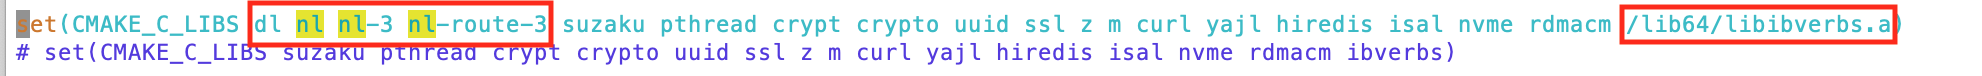
\includegraphics[width=10cm]{../imgs/cmake-link-static.png}
\end{center}

生成静态库
\begin{myeasylist}{itemize}
& SHARED  -> STATIC
& LIBRARY -> ARCHIVE
\end{myeasylist}

\section{gdb}

\begin{myeasylist}{itemize}
& ~/.gdbinit
& info registers
& info sharedlibrary
& gdb -p
\end{myeasylist}

gdb -p发现了mbuffer\_writefile进入死循环,原因是count==0。

猜想是重入了一个锁。

\section{wireshark}

\chapter{FlowChart}

% 流程图定义基本形状
\tikzstyle{startstop} = [rectangle, rounded corners, minimum width=3cm, minimum height=1cm,text centered, draw=black, fill=red!30]
\tikzstyle{io} = [trapezium, trapezium left angle=70, trapezium right angle=110, minimum width=3cm, minimum height=1cm, text centered, draw=black, fill=blue!30]
\tikzstyle{process} = [rectangle, minimum width=3cm, minimum height=1cm, text centered, draw=black, fill=orange!30]
\tikzstyle{decision} = [diamond, minimum width=3cm, minimum height=1cm, text centered, draw=black, fill=green!30]
\tikzstyle{arrow} = [thick,->,>=stealth]

\begin{tikzpicture}[node distance=2cm]
%定义流程图具体形状
\node (start) [startstop] {Start};
\node (in1) [io, below of=start] {Input};
\node (pro1) [process, below of=in1] {Process 1};
\node (dec1) [decision, below of=pro1, yshift=-0.5cm] {Decision 1};
\node (pro2a) [process, below of=dec1, yshift=-0.5cm] {Process 2a};
\node (pro2b) [process, right of=dec1, xshift=2cm] {Process 2b};
\node (out1) [io, below of=pro2a] {Output};
\node (stop) [startstop, below of=out1] {Stop};

%连接具体形状
\draw [arrow](start) -- (in1);
\draw [arrow](in1) -- (pro1);
\draw [arrow](pro1) -- (dec1);
\draw [arrow](dec1) -- (pro2a);
\draw [arrow](dec1) -- (pro2b);
\draw [arrow](dec1) -- node[anchor=east] {yes} (pro2a);
\draw [arrow](dec1) -- node[anchor=south] {no} (pro2b);
\draw [arrow](pro2b) |- (pro1);
\draw [arrow](pro2a) -- (out1);
\draw [arrow](out1) -- (stop);
\end{tikzpicture}

%作者:红伞菌
%链接:https://www.zhihu.com/question/20854046/answer/16400909
%来源:知乎
%著作权归作者所有。商业转载请联系作者获得授权,非商业转载请注明出处。
%作者:红伞菌
%链接:https://www.zhihu.com/question/20854046/answer/16400909
%来源:知乎
%著作权归作者所有。商业转载请联系作者获得授权,非商业转载请注明出处。

% Defines a `datastore' shape for use in DFDs.  This inherits from a
% rectangle and only draws two horizontal lines.
\makeatletter
\pgfdeclareshape{datastore}{
  \inheritsavedanchors[from=rectangle]
  \inheritanchorborder[from=rectangle]
  \inheritanchor[from=rectangle]{center}
  \inheritanchor[from=rectangle]{base}
  \inheritanchor[from=rectangle]{north}
  \inheritanchor[from=rectangle]{north east}
  \inheritanchor[from=rectangle]{east}
  \inheritanchor[from=rectangle]{south east}
  \inheritanchor[from=rectangle]{south}
  \inheritanchor[from=rectangle]{south west}
  \inheritanchor[from=rectangle]{west}
  \inheritanchor[from=rectangle]{north west}
  \backgroundpath{
    %  store lower right in xa/ya and upper right in xb/yb
    \southwest \pgf@xa=\pgf@x \pgf@ya=\pgf@y
    \northeast \pgf@xb=\pgf@x \pgf@yb=\pgf@y
    \pgfpathmoveto{\pgfpoint{\pgf@xa}{\pgf@ya}}
    \pgfpathlineto{\pgfpoint{\pgf@xb}{\pgf@ya}}
    \pgfpathmoveto{\pgfpoint{\pgf@xa}{\pgf@yb}}
    \pgfpathlineto{\pgfpoint{\pgf@xb}{\pgf@yb}}
 }
}
\makeatother
\begin{center}
\begin{tikzpicture}[
  font=\sffamily,
  every matrix/.style={ampersand replacement=\&,column sep=2cm,row sep=2cm},
  source/.style={draw,thick,rounded corners,fill=yellow!20,inner sep=.3cm},
  process/.style={draw,thick,circle,fill=blue!20},
  sink/.style={source,fill=green!20},
  datastore/.style={draw,very thick,shape=datastore,inner sep=.3cm},
  dots/.style={gray,scale=2},
  to/.style={->,>=stealth',shorten >=1pt,semithick,font=\sffamily\footnotesize},
  every node/.style={align=center}]

  % Position the nodes using a matrix layout
  \matrix{
    \node[source] (hisparcbox) {electronics};
      \& \node[process] (daq) {DAQ}; \& \\

    \& \node[datastore] (buffer) {buffer}; \& \\

    \node[datastore] (storage) {storage};
      \& \node[process] (monitor) {monitor};
      \& \node[sink] (datastore) {datastore}; \\
  };

  % Draw the arrows between the nodes and label them.
  \draw[to] (hisparcbox) -- node[midway,above] {raw events}
      node[midway,below] {level 0} (daq);
  \draw[to] (daq) -- node[midway,right] {raw event data\\level 1} (buffer);
  \draw[to] (buffer) --
      node[midway,right] {raw event data\\level 1} (monitor);
  \draw[to] (monitor) to[bend right=50] node[midway,above] {events}
      node[midway,below] {level 1} (storage);
  \draw[to] (storage) to[bend right=50] node[midway,above] {events}
      node[midway,below] {level 1} (monitor);
  \draw[to] (monitor) -- node[midway,above] {events}
      node[midway,below] {level 1} (datastore);
\end{tikzpicture}
\end{center}

\begin{figure}[htb]
\centering
%定义形状样式
\tikzstyle{startstop} = [rectangle, rounded corners, minimum width = 3cm, minimum height = 0.7cm, text centered, draw = black]
\tikzstyle{startstop2} = [rectangle, rounded corners, minimum width = 13cm, minimum height = 0.7cm, text centered, draw = black]
\tikzstyle{io} = [trapezium, trapezium left angle = 30, trapezium right angle = 150, minimum width = 3cm, text centered, draw = black, fill = white]
\tikzstyle{io2} = [trapezium, trapezium left angle = 30, trapezium right angle = 150, minimum width = 2.5cm, draw = black, fill = white]
\tikzstyle{io3} = [trapezium, trapezium left angle = 30, trapezium right angle = 150, minimum width = 2cm, draw = black, fill = white]
\tikzstyle{process} = [rectangle, minimum width = 3cm, minimum height = 1cm, text centered, draw = black]
\tikzstyle{decision} = [diamond, minimum width = 3cm, minimum height = 1cm, text centered, draw = black]
\tikzstyle{arrow} = [thick, -, >= stealth]
\tikzstyle{arrow2} = [thick, ->, >= stealth]

\begin{tikzpicture}[node distance = 1.5cm]
% 定义流程图具体形状
\coordinate[label = left:{\small 输入图像}](A) at(-1.5, 0);
\node(in1) [io] {};
\node(pro1) [startstop, below of = in1] {\small 线性滤波};

\node(in2 - 2)[io3, below of = pro1, yshift = -0.6cm]{};
\node(in3 - 2)[io3, left of = in2 - 2, xshift = -2.5cm]{};
\node(in4 - 2)[io3, right of = in2 - 2, xshift = 2.5cm]{};

\node(in2 - 1)[io2, below of = pro1, yshift = -0.3cm]{};
\node(in3 - 1)[io2, left of = in2 - 1, xshift = -2.5cm]{};
\node(in4 - 1)[io2, right of = in2 - 1, xshift = 2.5cm]{};

\node(in2) [io, below of = pro1] {\small 颜色};
\node(in3)[io, left of = in2, xshift = -2.5cm]{\small 亮度};
\node(in4)[io, right of = in2, xshift = 2.5cm]{\small 方向};

\node(in5)[startstop2, below of = in2 - 2]{\small Center - Surround差异计算及归一化};

\node(in6 - 2)[io3, below of = in5, yshift = -0.6cm]{};
\node(in7 - 2)[io3, left of = in6 - 2, xshift = -2.5cm]{};
\node(in8 - 2)[io3, right of = in6 - 2, xshift = 2.5cm]{};

\node(in6 - 1)[io2, below of = in5, yshift = -0.3cm]{};
\node(in7 - 1)[io2, left of = in6 - 1, xshift = -2.5cm]{};
\node(in8 - 1)[io2, right of = in6 - 1, xshift = 2.5cm]{};

\node(in6) [io, below of = in5] {};
\node(in7)[io, left of = in6, xshift = -2.5cm]{};
\node(in8)[io, right of = in6, xshift = 2.5cm]{};

\coordinate[label = left:{\small 特征图}](B) at(-1, -6.2);
\coordinate[label = left:{\small (12张)}](C) at(-1.5, -7.5);
\coordinate[label = left:{\small (6张)}](D) at(2.7, -7.5);
\coordinate[label = left:{\small (24张)}](E) at(6.7, -7.5);

\node(in9)[startstop2, below of = in6 - 2]{ \small 跨尺度合并及归一化 };

\node(in10) [io, below of = in9] {};
\node(in11)[io, left of = in10, xshift = -2.5cm]{};
\node(in12)[io, right of = in10, xshift = 2.5cm]{};

\coordinate[label = left:{\small 醒目图}](F) at(-1, -9.5);
\node(in13) [startstop, below of = in10] {\small 线性组合};
\node(in14) [io, below of = in13] {};
\coordinate[label = left:{\small 显著图}](G) at(-1, -13);

\node(in15) [startstop, below of = in14] {\small 赢者取全};
\coordinate[label = left:{\small 显著位置}]() at(1, -16.1);
\coordinate[label = left:{\small 反馈抑制}]() at(4.5, -14.7);

%连线
\draw[arrow](pro1) -- (in1);
\draw[arrow](pro1) -- (in2);
\draw[arrow](pro1) -- (in3);
\draw[arrow](pro1) -- (in4);
\draw[arrow](0, -4.75) -- (in2 - 2);
\draw[arrow](-4, -4.75) -- (in3 - 2);
\draw[arrow](4, -4.75) -- (in4 - 2);
\draw[arrow](0, -5.45) -- (in6);
\draw[arrow](-4, -5.45) -- (in7);
\draw[arrow](4, -5.45) -- (in8);
\draw[arrow](0, -8.35) -- (in6 - 2);
\draw[arrow](-4, -8.35) -- (in7 - 2);
\draw[arrow](4, -8.35) -- (in8 - 2);
\draw[arrow](0, -9.05) -- (in10);
\draw[arrow](-4, -9.05) -- (in11);
\draw[arrow](4, -9.05) -- (in12);
\draw[arrow](in13) -- (in10);
\draw[arrow](in13) -- (in11);
\draw[arrow](in13) -- (in12);
\draw[arrow](in13) -- (in14);
\draw[arrow](in14) -- (in15);
\draw[arrow](in15) -- (0, -15.8);
\draw[arrow](0, -15.4) -- (2.5, -15.4);
\draw[arrow](2.5, -14) -- (2.5, -15.4);
\draw[arrow2](2.5, -14) -- (0, -14);
\end{tikzpicture}
\caption{IT算法流程\cite{Itti}}
\end{figure}

% 设置颜色代号
\colorlet{lcfree}{green}
\colorlet{lcnorm}{blue}
\colorlet{lccong}{red}
% -------------------------------------------------
% 设置调试标志层
\pgfdeclarelayer{marx}
\pgfsetlayers{main,marx}
% 标记坐标点的宏定义。交换下面两个定义关闭。
\providecommand{\cmark}[2][]{%
  \begin{pgfonlayer}{marx}
    \node [nmark] at (c#2#1) {#2};
  \end{pgfonlayer}{marx}
  } 
\providecommand{\cmark}[2][]{\relax} 
% -------------------------------------------------
% 开始绘图
\begin{figure}[h]
\centering
\scalebox{.8}{                  %设置缩放	
\begin{tikzpicture}[
    >=triangle 60,              % 箭头的形状
    start chain=going below,    % 从上往下的流程
    node distance=6mm and 60mm, % 全局间距设置
    every join/.style={norm},   % 连接线的默认设置
    ]
% ------------------------------------------------- 
% 节点的样式定义 
% <on chain> 和 <on grid> 可以减少手动调整节点位置的麻烦
\tikzset{
  base/.style={draw, on chain, on grid, align=center, minimum height=4ex},
  proc/.style={base, rectangle, text width=8em},
  test/.style={base, diamond, aspect=2, text width=5em},
  term/.style={proc, rounded corners},
  % coord 用来表示连接线的转折点
  coord/.style={coordinate, on chain, on grid, node distance=6mm and 25mm},
  % nmark 用来表示调试标志
  nmark/.style={draw, cyan, circle, font={\sffamily\bfseries}},
  % -------------------------------------------------
  % 不同的连接线样式
  norm/.style={->, draw, lcnorm},
  free/.style={->, draw, lcfree},
  cong/.style={->, draw, lccong},
  it/.style={font={\small\itshape}}
}
% -------------------------------------------------
% 先放节点
\node [term, densely dotted,fill=lccong!25, it] (p0) {输入};
% 用 join 表示和上一个节点相连 
\node [proc, join]	{使用非线性最小二乘法得到 $X_0$};
\node [proc, join]	{记录 $X=X_0, f=f(X_0)$};
\node [test, join] (t1)	{$T>T_E$?};
\node [proc] (p1)		{$step=0$};
\node [test, join] (t2)	{$step<count$?};
\node [proc] (p2)		{得到新状态$P_N=P+scale\times rand$,计算目标函数差$\Delta f$};
\node [test, join] (t3)	{$F_{Accept}<rand$?};
\node [proc] (p3)		{记录新状态 $X=X_N,f=f(X_N)$};

\node [proc, left=of t1] (p4)	{$T=T\times a,scale=scale\times b$};
\node [term, densely dotted, right=of t1,fill=lcfree!25](p5)	{输出};
\node [proc, right=of t3](p6)	{$step++$};

\node [coord, left=of t2] (c1)  {}; 
\node [coord, right=of t2] (c2)  {}; 
\node [coord, right=of p3] (c3)  {}; 
%先画南北方向的连接线,先画线再画两端的标志和箭头
\path (t1.south) to node [near start, xshift=1em] {$y$} (p1);
  \draw [*->,lcnorm] (t1.south) -- (p1);
\path (t2.south) to node [near start, xshift=1em] {$y$} (p2);
  \draw [*->,lcnorm] (t2.south) -- (p2);
\path (t3.south) to node [near start, xshift=1em] {$y$} (p3);
  \draw [*->,lcnorm] (t3.south) -- (p3);
%接着画东西方向的连接线,方法同上
\path (t1.east) to node [near start, yshift=1em]  {$n$}(p5);
  \draw [o->,lcnorm] (t1.east) -- (p5);
  \draw [->,lcnorm] (p4.east) -- (t1);
\path (t3.east) to node [near start, yshift=1em]  {$n$}(p6);
  \draw [o->,lcnorm] (t3.east) -- (p6);
\path (t2.west) to node [near start, yshift=1em]  {$n$}(c1);
  \draw [o->,lcnorm] (t2.west) -- (c1) -| (p4);
  \draw [->,lcnorm] (p3.east) -- (c3) -| (p6.south);
  \draw [<-,lcnorm] (t2.east) -- (c2) -| (p6.north);
\end{tikzpicture}
}
\label{fig:algorithm}
\end{figure}

\tikzstyle{every node}=[draw=black,thick,anchor=west]
\tikzstyle{selected}=[draw=red,fill=red!30]
\tikzstyle{optional}=[dashed,fill=gray!50]
\begin{tikzpicture}[%
  grow via three points={one child at (0.5,-0.7) and
  two children at (0.5,-0.7) and (0.5,-1.4)},
  edge from parent path={(\tikzparentnode.south) |- (\tikzchildnode.west)}]
  \node {texmf}
    child { node {doc}}
    child { node {fonts}}
    child { node {source}}
    child { node [selected] {tex}
      child { node {generic}}
      child { node [optional] {latex}}
      child { node {plain}}
    }
    child [missing] {}
    child [missing] {}
    child [missing] {}
    child {node {texdoc}};
\end{tikzpicture}

\begin{tikzpicture}[sibling distance=10em,
    every node/.style = {shape=rectangle, rounded corners,
        draw, align=center,
        top color=white, bottom color=blue!20}]]
        \node {root}
        child { node {snap1} }
        child { node {snap2}
            child { node {snap3}
                child { node {snap4} }
                child { node {snap5} }
                child { node {snap6} } }
            child { node {snap7} } };
\end{tikzpicture}

\begin{tikzpicture}
  \begin{scope}[blend group = soft light]
    \fill[red!30!white]   ( 90:1.2) circle (2);
    \fill[green!30!white] (210:1.2) circle (2);
    \fill[blue!30!white]  (330:1.2) circle (2);
  \end{scope}
  \node at ( 90:2)    {Typography};
  \node at ( 210:2)   {Design};
  \node at ( 330:2)   {Coding};
  \node [font=\Large] {\LaTeX};
\end{tikzpicture}

% Drawing part, node distance is 1.5 cm and every node
% is prefilled with white background
\begin{tikzpicture}[node distance=1.5cm,
    every node/.style={fill=white, font=\sffamily}, align=center]
  % Specification of nodes (position, etc.)
  \node (start)             [activityStarts]              {Activity starts};
  \node (onCreateBlock)     [process, below of=start]          {onCreate()};
  \node (onStartBlock)      [process, below of=onCreateBlock]   {onStart()};
  \node (onResumeBlock)     [process, below of=onStartBlock]   {onResume()};
  \node (activityRuns)      [activityRuns, below of=onResumeBlock]
                                                      {Activity is running};
  \node (onPauseBlock)      [process, below of=activityRuns, yshift=-1cm]
                                                                {onPause()};
  \node (onStopBlock)       [process, below of=onPauseBlock, yshift=-1cm]
                                                                 {onStop()};
  \node (onDestroyBlock)    [process, below of=onStopBlock, yshift=-1cm] 
                                                              {onDestroy()};
  \node (onRestartBlock)    [process, right of=onStartBlock, xshift=4cm]
                                                              {onRestart()};
  \node (ActivityEnds)      [startstop, left of=activityRuns, xshift=-4cm]
                                                        {Process is killed};
  \node (ActivityDestroyed) [startstop, below of=onDestroyBlock]
                                                    {Activity is shut down};     
  % Specification of lines between nodes specified above
  % with aditional nodes for description 
  \draw[->]             (start) -- (onCreateBlock);
  \draw[->]     (onCreateBlock) -- (onStartBlock);
  \draw[->]      (onStartBlock) -- (onResumeBlock);
  \draw[->]     (onResumeBlock) -- (activityRuns);
  \draw[->]      (activityRuns) -- node[text width=4cm]
                                   {Another activity comes in
                                    front of the activity} (onPauseBlock);
  \draw[->]      (onPauseBlock) -- node {The activity is no longer visible}
                                   (onStopBlock);
  \draw[->]       (onStopBlock) -- node {The activity is shut down by
                                   user or system} (onDestroyBlock);
  \draw[->]    (onRestartBlock) -- (onStartBlock);
  \draw[->]       (onStopBlock) -| node[yshift=1.25cm, text width=3cm]
                                   {The activity comes to the foreground}
                                   (onRestartBlock);
  \draw[->]    (onDestroyBlock) -- (ActivityDestroyed);
  \draw[->]      (onPauseBlock) -| node(priorityXMemory)
                                   {higher priority $\rightarrow$ more memory}
                                   (ActivityEnds);
  \draw           (onStopBlock) -| (priorityXMemory);
  \draw[->]     (ActivityEnds)  |- node [yshift=-2cm, text width=3.1cm]
                                    {User navigates back to the activity}
                                    (onCreateBlock);
  \draw[->] (onPauseBlock.east) -- ++(2.6,0) -- ++(0,2) -- ++(0,2) --                
     node[xshift=1.2cm,yshift=-1.5cm, text width=2.5cm]
     {The activity comes to the foreground}(onResumeBlock.east);
\end{tikzpicture}


\part{历史}

\chapter{2012}

10月,从美地森离职去光点图论,接触移动互联网技术:

\begin{enumbox}
\item Nginx
\item Redis
\item MongoDB
\item ElasticSearch
\item Hadoop/HBase
\end{enumbox}

性能优化:
\begin{enumbox}
\item 增加MongoDB index
\item 增加多级缓存,包括Nginx/App/Redis等
\end{enumbox}


\chapter{2016}

FusionStor

\begin{enumbox}
\item 远程复制
\item 一致性卷组
\item EC
\item COW snaptree
\item LSV (2017)
\end{enumbox}


\chapter{2017}

深入FusionStor实现



\chapter{2018}

华云网际,分布式块存储系统开发。

\section{08}

\subsection{01}

dmidecode可以查询服务器型号

\subsection{02}

理解target,各种各样的target。host-target之间的transport和protocol是区分的关键。
\hl{类比TCP协议栈}去理解各种新的网络技术。

tgtctl是target和storage的交接点,体现在文件\hl{nvmf\_suzaku\_io}里。

spdk的NVMf导出bdev。如何对接分布式存储?

把libnvme用git管理起来\todo{git-libnvme}。

尝试用一台vm把suzaku跑起来。看看具体要求和配置是什么?

完善关键流程,补上漏洞。采用\hl{用系统来工作}的理念,完善过程。

test是什么状态?应该怎么做?

hazard相关文档。

排兵布阵,上知天文下知地理。

NVMe中buffer的表示,sge?

\subsection{06}

通过ipmi控制服务器。

一块nvme盘加不上,不知为什么?51,52,53上都是如此。51重新插拔盘解决,52、53拔掉电源,重启解决。

实则性能不如8.1版,为什么?观察到disk延迟高,对disk单独进行性能测试,剔除慢盘。
用4盘测试,性能达到600w+,但latency double了。

测量每块盘的平均队列深度和延时。为什么disk的latency突然变大了呢?
\begin{myeasylist}{itemize}
& 没有读过的盘,非稳态性能?
& bactl有问题?
& remote first后,iops显著下降,latency显著升高,磁盘压力小
& \hl{把单卷大小改为80G之后,性能提升上去了}。
\end{myeasylist}

mds\_rpc\_paget,并发高,导致rangectl的内存耗尽?

加入节点,rehash,等待lease timeout,io会中断。

三个client不要同时启动,而是错开几秒钟。

rdma 在提交和完成之间,可能会占用大量内存,导致内存耗尽。怎么解决?
内存不足时使用后备内存,以处理峰值情况。或者core内存管理动态化。

\hl{拆分为两个库,都需要用静态库},不能用so。

\subsection{07}

\subsection{08}

\subsection{09}


\section{201809}

\subsection{0901}

\subsection{0902}

\subsection{0903}

战略几何学、神圣几何:圆是时间,四方形、十字架是空间,三角形是存在,构成时-空-存在的结构。

双环系统可以解释一切,双环相交处是太极图。右手螺旋法则。

周末读书,关注到几个概念,心神、机发,心神论是黄帝内经的精髓,机发论是易道主义的理论枢纽。

机是什么?随机而动,机是变动不居的存在,但可以通过思维与实践的方式去认识和把握。
阳明心学的精髓:此心不动,随机而动,就是圆点结构。

一心一意到专业学习上,有道有术两个层次多个层次。所有的事情,都是培养心体。
要留出足够的时间去反思,并记录下反思的过程与结论。

这么多年,很遗憾的一点就是不能一心一意,也就是不诚,身在曹营心在汉,不能全心全力地投入到手头要紧的事情上,
老是觉得另有更大价值的事情,反而导致手头的机会也白白溜走。

今后当从容规划(转动PDCA循环),稳扎稳打,一步一个脚印,去实现目标。

几有多义,主要是微和危。事物的萌芽状态,看不透、想不明白,\hl{惟精是惟一的功夫},博文是约礼的功夫。这是阳明一贯的主张。
守住底线、抓住关键是方法,围绕一转动PDCA循环。

\hl{如何尽快实现财务自由}?四象限,打工、个体户、创业、投资。贯穿其中的是\hl{专业、工匠精神}。
只是有工匠精神依然不够,要有道。立足于当下,什么才是最重要的事情呢?

\hl{乾之九三给出了答案}。乾坤是易的门户,黄帝垂衣裳而治天下,盖取诸乾坤。

\subsection{0904}

乾坤是易的门户,易是通向现实世界的门户。这是非常重要的论断,因为一是学易之法,二是用易之法,学以致用,解决现实问题。
读书不在乎多,学宗大易,一部易经观天下。透过一部易经,而通达于现实世界,得偿所愿,心想事成。
通过易,撑起开物成务、进德修业的英雄梦想之旅。

六爻之动,三极之道。分而论之,初二为地道,三四为人道,五上为天道,匹配几、诚、神。

用\hl{三级火箭模型}分析创业公司的发展轨迹和着力点,什么是发动机?如何一环套一环?
产品和客户是任何公司的两极。设计理念与客户反馈要综合为用。

易之三义,变易、不易、易简。

\subsection{0905}

努力经营事业,开始物色各类人选,看看水浒传、三国演义,任何事业都不会想当然地一蹴而就,而是长期经营的结果。
事业是男人的第一支柱。

易经在这方面有着深沉的诉求,圣人以神道设教,抛开迷信的成分,易经是第一励志书,也是第一帝王书。
学习易经,方术方面了解即可,不作为主要方面,重要的是开物成务、进德修业方面的启发和辅助。

至九四,始入于上层,开启了自己的平台和事业。上下分际处是着力点。
或跃在渊,此一跃是多方面因素叠加的结果,主要还在于自己的野心、理念、认知。
此一跃,不回头。

一是因果律,二是神圣意志之发扬。乾卦就是这样的精神力量,乘云气而御飞龙,高扬进取意识。

更加open地去思考关键问题,包括行业、事业等等。思考、交流都是需要的。
进一步去了解别的产品,主要是把握趋势。

双环系统可以解释一切,双环相交处是太极图。

怎么通向现实世界呢?

\subsection{0906}

不能控制自己的情绪,太幼稚,这种东西纯粹影响发挥。当前第一要务是什么?事业,不容置疑。迄今没有起色。

第一个是专业环,这是安身立命之本。经过多年的摸索,是整理收割的时候了。

第二个是易经,全面拥抱易经,以之作为进德修业的重要基础。以此洗心,退藏于密,洗心,就是淬炼心智模式。
易经在思维方面,有着深度与广度。进入眼界的思维模型,都挂入易经这个思维格栅中去,易经就是太上老君的八卦炉,
淬炼出了孙悟空的火眼金睛。

另外,黄帝内经所蕴含的神本论以及机发论思想,在易经中也有深入的体现。洁净精微,易之教也。

环环相扣,专业与易经之环,碰撞出火花。工作与生活都需要大设计。

不要急、慢慢来。易经为起点,一部易经观天下,指导生活与工作之设计。专业是工作的一部分。
生活是进德,工作是修业,内外兼备,合内外,一物我。

一切的学习都不仅仅为了学习而学习,为了单纯的知识而学习,而是为了解决问题。

关键思想:
\begin{enumbox}
\item 确定易经作为最高指导思想,第三空间或虚或实,主要指的是这个,过有原则的生活,富有之谓大业、日新之谓盛德
\item PDCA作为执行方法
\item 双环系统分别对应生活和工作
\item 把\hl{视点/视角方法}作为架构描述语言
\item B:确定把分布式存储作为主要的技术领域
\item B:确定把QoS作为主要的研究方向之一
\end{enumbox}

\subsection{0911}

全力以赴到专业方向上,去解决关键问题,太极云尔,是反思框架。

心、道、物的三合之道,适合于下一阶段的学习过程。心就是阳明所谓良知,为学头脑所在,多问多思。道,原则,方法论,架构。
物是要研究的系统,要解决的问题。以道观之,以架构之眼看系统,当如庖丁解牛。

双环,一者三合之道,二者PDCA。双环正交?

对解决问题有腻烦心理,问题是前进的动力,当善待之,乐于去搞定她。

\subsection{0912}

心神主宰,以道观之,落实到物,以道的光华普照世界。寂然不动、感而遂通天下之故,这是二重性。

第一个小目标,100w,1000w,以此类推。明年大概就有100w了,坚定地走下去,不急不躁。重为轻根,静为躁君。

架构驱动的软件开发过程。

坚持用SWOT分析,是战略分析的起步。

\hl{本周末给出一个更明确的路线图}。第一,强化架构思维能力,视图视角是标准做法,IEEE STD 1471-2000。
视图可以视点集为模板,也可以单独定义。运用视角到视图之中,形成纵横交错的架构描述。

\subsection{0913}

\begin{shadequote}

能把诚神几统一起来的为圣人。北宋周敦颐在《通书》中提出的命题。“寂然不动者,诚也。感而遂通者,神也。
动而未形,有无之间者,几也。……诚神儿曰圣人”(《通书·圣》)。
诚是静无的,即“诚无为”(《通书·诚几德》)。神“感而遂通”,是诚的直接表现。几处于静无动有之间,是动之始。
诚是纯粹至善的,是一切道德行为的源泉。
神是诚的直接表现,故亦善。只有几“动于彼”,感外物而动,故兼有善恶。
《宋元学案·濂溪学案上》云:“常人之心,首病不诚。不诚故不儿而著。不几故不神。物焉而已。”
常人不能以诚贯几,受物之累而为恶。只有圣人才能以诚贯几,去几中之恶,把诚神几统一起来,故诚神几曰圣人。
\end{shadequote}

心道物,诚神几,有对应关系。把心置于三角形顶点处,似更体贴。

养心莫善乎诚,致诚则无它事。至诚之道,可以前知。惟天下至诚,为能经纶天下之大经,立天下之大本,成天地之化育。

圣人以神道设教,道则通神,一阴一阳之谓道,阴阳不测之谓神。何为神?妙万物而为言者。

几,人心惟危,道心惟微,几则合多义而言。机发论更提出制机的说法,乃易道主义的理论枢纽。
从机发论的角度理解,\hl{黄帝内经}灵枢,\hl{鬼谷子、阴符经}亦然。

\hl{此三角形居于左侧(符合右手螺旋法则),圆形+十字架构成的几何形状居于右侧(SWOT, PDCA, 2x2矩阵及其延伸,符合左手螺旋法则),
左右交错,形成太极之两仪}。大拇指都指向自己,反求诸己,建立自我,贵我通今,时变是守。
此参伍以变,错综其数的义理架构,实有进一步发挥的余地。

左为知、右为行,以此类推,大商之道的道术、变常、方圆、生死、利害、取予之对立统一,也是如此。

孙正义的25字诀,与\hl{周易、兵经百字、东方战略学},都是以字通道的卓越理念。

\subsection{0914}

观象玩辞,以字通道。建勋画论的三合之道,启人深思。道具太极位,则有商讨的余地。邵雍曰:心者太极也。华严经云:心如工画师,能画诸世间。
阳明心学也是如此。心是能动的一面,也是目的性的一面,使心居于太极位,乃应有之义。心秉道通物,心格物穷理,天性,人也,人心,机也。
立天之道,以定人也。此说并不否定或拉低道的价值,而是在建立自我的阶段,高扬心性,确立为学的头脑。道依然是那个道,
致吾心之良知于事事物物,则事事物物皆得其理。即满足了目的性要求,又满足了道的约束性原则性。

欲正其心者,先诚其意。在明道、格物的过程中,诚其意。事上磨练,皆在涵养此心之体。由物及心,完成此逆时针的环转关系。此右手螺旋法则。

如忽略道的环节,而直奔物的主题,则易于陷入事务主义的泥淖之中,事半功倍,乃至无功而返。
如过于强调理论,也有教条主义的倾向。

神者生之本。

\subsection{0918}

系统思考。

职场与理想的距离,靠三度修炼去完成。三度:态度、气度、厚度。读一艮卦,胜读一部华严。
中秋看王明夫主编的三度修炼,好好想一想下一步的规划。

\subsection{0920}

离开HY的可能较大,离不离开,都要以成长为主要标准。时间并不充裕,接下来到年底的一段时间,好好锤炼专业技能。

\hl{优先考虑开启自己的事业},专业技能的学习、知识体系的构建,不能脱离这个目的,才称得上学以致用。

\hl{全闪时代来临,离自己最近,怎能再次错过}?应采用包围式学习,地毯式学习,既要明确关键,又要面面俱到,点线面体,全面展开。

在多副本复制的场景下,由一控制器负责,如果控制器发生切换,则开启新纪元。在某一控制器的生存期内,
每次提交采用单调递增的版本号,所以二元序号的构成:(epoch, version/clock)。
卷控制器可管理很多chunk及其副本一致性,控制器位置与副本位置不具有对应关系。\hl{卷控制器可迁移}。

关于控制器的若干关键问题:
\begin{enumbox}
\item 如何选取控制器
\item 客户端如何定位控制器
\item 控制器发生切换又如何
\end{enumbox}

paxos的精髓是温故知新,一个实例产生一个值。如何标记序号?序号可以是二元结构,方便处理。

multi paxos与RAFT的异同?每一个控制器的生命周期包括三阶段:\hl{选主、恢复、正常操作}。

进一步,传统的2PC、3PC算法的不足和使用场景。这类算法是分布式系统的精髓,务必加以消化理解。

\hl{算法是程序员的金线},理应是下一阶段的重点。比如,通过token bucket或leaky bucket解决qos问题,实现很简单,设计很精妙。

马云定随舍三部曲,第一曲是定字诀。艮,止也。知止而后有定,定而后能静。

\hl{起居有常、饮食有节},乃养生之道,不仅此也,常与节有深意存焉。
财自道生、利缘义取,是大商之道。菩萨畏因,凡夫畏果。

\hl{多听多问}是领导之道,陈述句不如疑问句。

易经的卦图是直线,加上圆点哲学,三角形集两者之大成,融合双线法则、圆点哲学、三点论、一分为三诸论而为一,
算是多年思考、探索的一点结论。三生万物,由此而展开其广泛的运用过程,进入明体达用的第二阶段。
用太极两仪模式解读三角形各点之间的关系。

道是吾观物的门户、工具,不能僭越心的第一性,道物、道器、体用,分阴分阳,叠用柔刚。
\hl{吾有方圆之形}。五代表圆点哲学,PDCA等。以五为食,哈?口为口、为目,以五观之、观天下。

两个三角形,下一个代表物理资源,上一个代表虚拟资源,中间的交点是集群,物理资源总而为一,进一步生化出虚拟资源。

心道物三角,自身也有两种旋转方向,左手螺旋右手螺旋,标准图以心为顶点。

\subsection{0920}

战略一二三,美团十字架,参伍点成圆,乱环诀中诀。

智仁勇三达德,好学近乎智,力行近乎仁,知耻近乎勇。

在乱环之中,存在第一义,找到她!

架构、算法是内功心法,练拳不练功,到老一场空。

功业之心热灼,怎么开始?如何播种下第一粒种子?离什么最近? 立于中央,由近及远。

无所待,此时就是开始!此时此地,从心开始。

开始不难,终局判断如何?商业计划书?开始吧。

人钱事,搭班子、定战略、带队伍。做什么?怎么做?如何解决启动资金的问题?

如何整合资源?一二三级火箭分别是什么?

\subsection{0925}

心道物,以心为开始,以道为顶点,以物为落实。三者太极两仪,环转无尽,融归与太极大道之中。
如此排列,不压抑心的能动创造性和塑造能力。

心何以转物?以道为中介,诚神几,修心贵诚,通道故神,风起于青萍之末,挥之于泰山之本。
上通于道,下及于物。向道的跃迁层层递进,进一层有一层的道理。

任何一点都不足以表达正确的关系。

中秋假期间一个最重要的反思就是要有制胜的意志。\hl{善用兵者,修道而保法,故能为胜败之政}。
举凡人事百端,无不以胜或赢为最终的目的。取胜的方法多端,宗旨则一。

古今中外的人之共识,老庄虽然一直在说恬淡虚无,何尝忘记求以得,有罪以免也,故为天下贵。

从胜的角度,从修身为本三合之道的角度去诠释经典,别有一番风韵。

\hl{立足于专业技能,从战略的角度拓展未来成长空间},战略思维是一项极端重要的能力。

道天地将法,也是一重要的思考框架。尚五,五包含了一二三四,圆点哲学、太极阴阳、三才之道、四象/PDCA。

老子缺少点进取的意味,孙子则攻守兼备。

心到道的距离是认知差,\hl{道是超认知}。在不同的认识面上,相同的公理具有不同的内核,这就是hegel一直说的熟知非真知。
以道观之,在道的高度上,运用简单而普适的公理,可以达到非常好的结果。

人心惟危,道心惟微。危是指称思维的不可靠,微则是思维的神妙不测,真理与谬误在一线之间。
洞察思维的误区盲点,极深研几,就可以越来越接近道的境界。

查理芒格研究思维的错误模式,就是有鉴于此。普通的思维是靠不住的。
波普尔的证伪理论,索罗斯的反身性,都是解决这一问题的哲学努力。
更早,则有休谟的因果质疑。

\hl{枕戈待旦、厉兵秣马},为了最后之胜利,不能不如此。

心的综合能力,读书如果不思考,就破坏了这种能力,显得支离。

为什么要从心开始呢?虚心涵泳,切己体察。

架构师,工匠精神,粟裕尽打神仙仗。\hl{全力以赴投入到专业技能的学习和提升上去},主次不能颠倒。
说别的事情还显得太远,比如和君的国势、产业、资本、管理四库全书等。这是下一阶段的事情。

通过研读阳明学,更主要的是,通过建勋的画道提出的三合之道,确立了基础的思想方法和工作方法。

破局、突破,更上一层楼。

进一步提出经营方针和工作程序。

\subsection{0926}

六经注我,我注六经。阳明学提升了我的价值,先确立我,建立自我,第二步才是追求无我之境。

系统读书,一旦确立了我,读书就是为我所用的过程。志于道,游于艺,六艺摄于一心,如此,心物关系中,心为主,物为从,精神作为能动性的一方面,发挥了更为重要的作用。
即是在格物中诚意,在诚意中格物,尊德性而道问学。

留给自己的大机会不多了,需要极大地发挥精神的能动性,去慎思明辨。四十不惑,处在这个关键的转折点,怎能不好好地把握呢?
机遇偏好有准备的头脑,潜龙勿用,一定要静下心来,苦练内功,打好下一步发展的坚实基础。

战略致胜,战略是道的运用,以道莅天下。孙子兵法计篇:道天地将法。以五行对照之,道立于中央,天地定位,左将右法。
将作为能动性的一方,也不能不受道的制约,取胜的一切要素,都围绕着道而旋转,五行是更具体的模型。道具有目的性和工具性等多重价值。

\hl{搭班子、定战略、带队伍}是柳传志的联想方法,对应到将、道、法横轴上。
将是领导、法是管理。国势、产业、资本、管理,管理是创业之后的事情,且不可过于陷入微观管理的泥潭。
产业才是第一要考虑的领域,在国势下定位产业,资本、管理是随着产业而运转的。

\hl{战略罗盘}从内外、知行两个维度进行划分,从外到内。

借力打力,分布式存储最好的借力点是openstack和vmware、oracle等场景。顺势而为,方可事半功倍。
不懂得借力,没有生态思维,自行其是,往往落个狼狈下场。

认识差:红山为什么看不到云才是最大的趋势?华云错失超融合、全闪风口。后果严重。为什么大家往往看不到最好的机会?

光点的机会又是在哪里?从手机壁纸到游戏、区块链?

确实到了一个关节点,在专业上提炼总结,来一个大突破。

\subsection{0927}

十一在家研读阳明心学,以及企业家精神。阳明心学是与三合之道最为合拍,源于易经和道德经古老传统的三合之道,源远流长。
数年探索终将有所结论,涓涓细流汇成汪洋大海。悟后起修,悟后大有功夫在。

白立新的致良知四合院是阳明心学研究的一股清流,面向企业家也是有的放矢。

也不要在书面材料里太久,反观自心是最后的归宿。明心、净心,万事万物即在其中了。扩大心量,笼罩万物。
心生则种种法生,六祖坛经:心量广大,犹如虚空。

从专业工作者,进阶到企业家、投资家,打通四象限,是毕生追求。经过多年沉淀,人生进入第二阶段,唤起使命。
千面英雄的轮回,乾卦六龙御天,皆指示了人生的阶段性、周期性。40-50岁,正值人生壮年,争取走完第二阶段。开启第三阶段。

向前看,扭转思维的主视角。六合上下,立足当下,展望未来。能做什么? 高瞻远瞩
复盘重要,未来更重要。禅剑合一,心剑合一。引入第三点道,层次分明,动静无间,则曲得其妙。

不是观众,演员,要去做导演。

\subsection{0928}

S曲线是成长曲线,第一曲线跨越到第二曲线靠什么? 不要忘了当下最重要的目标,自我成长!

在公司住了一宿,感觉尚可。创造这样的条件。研究以下生活自理方面的,极简主义风格,体现了根据地的重要性。
建立根据地,然后进可攻退可守,极大地拓展了生活工作的战略半径。

\hl{根据地思维}不仅是个人的,工作、创业等都需要,是一个重要的战略思维。
高筑墙、广积粮、缓称王,说白了,就是根据地思维。
建立根据地后,就保有了一个\hl{极具弹性的战略空间}。
在三国争霸、国共之争中都体现得淋漓尽致。

在北城买房、甚至在郊区买别墅是一个战略构想,解决工作与居住地之间距离的矛盾。
确实,90\%的问题是money的问题。财务自由是个人发展的一个重要里程碑。

专业上,\hl{分布式存储系统就是一个战略根据地}。

\hl{国庆节计划在家研读阳明心学与企业家精神},认真思考下一步的作战规划。
从作战的视角来审视各种活动,会有更大洞见。
作战追求胜利,评估得失成败的根本原因。兵之形象水,因地制宜的灵活性。随机而动,追求胜利。
任何活动,都是项目,也是一场战斗、战役、战争。
没有求胜的坚决意志,就会错过最美的风景。
阳明在军事上的成绩,与悟道有关,也与他研读兵学有关。

兵贵胜,不贵久。

读\hl{阳明心学的管理智慧},三体世界的提法,与三合之道契合。主体世界、本体世界、客体世界,与心道物一一对应。
心上通于道、下及于物,这个上下反复的过程,完成了三者的互联互通。

心即理,知行合一、致良知、四句教等核心命题都可以在三合之道框架下,得以完美诠释。
知行合一贯通三体世界,故有三知三行之说。

心、场、道、法、术、器,细化了心道物三要素,引入了程序化、结构化的元素,如原则、用系统来工作等书所提及的,
约法三章,修道而保法,故能为胜败之政。

互联网思维的贯通,\hl{S2B2C商业模式的解读},很有新意,值得进一步品味。

国庆细读。阳明心学与企业家精神,围绕这个中心问题来进行阅读。
企业家是第二阶段的主线,一定要好好体会这个角色面临的机遇和挑战。

现在处内外交困之境地,内则杂念憧憧,外则工作事业皆不尽如人意。
当思如何破局?向前看,战略六看!

应以阳明学为中心,一心摄六艺,六艺摄于一心,六经注我开生面。
易经乃一经一艺,\hl{心易}的说法,有共鸣。

\hl{阳明学是很好的下手处,切问近思}。在三合之道的义理框架下,理解阳明学变得容易多了。
重要的不仅仅是理解,更在于知行合一。\hl{且知且行,咬定青山不放松}。

\subsection{0929}

从阳明心学可以辐射到传统和当代的诸多领域,比如对明治维新的影响,阳明心学复兴的意义。
周易古奥,难以直接受用。阳明心学从解决心物关系问题入手,确立了心的主体地位(张学智会通中西古今)。

高扬主体精神,心与道合,道济天下,以道莅天下,知行合一。PDCA,规划是知,执行是行,检查是知,调节优化是行。知行并进。

知,认知差,超认知。知己知彼、百战不殆。知机而后制机,知在人生旅途中,发挥着巨大的作用。
吴军写见识,无战略悲人生,处处都在说明知的极端重要性。认识升级、培育正念,是人生要务。

预知、先见之明,更是重要素养。道知,以道而知。损兑,专以心眼察也。阅读、旅行等只是获取知的具体途径,
开发心田,培育正念,时时处处在心体上下功夫。

涵养须用敬,进学则在致知。敬字提点人心,使不昏沉放逸,精神内守,为功大矣。
不仅此也,\hl{离致知而言内守,则有枯寂之弊}。

以良知之体、道之光华照耀大千世界。

尽快挣到足够的钱,是当前最大目标。如何做到呢?在因上用力。

早上学习专业,晚上用阳明心学作为反思批判的心法,做此二元分解,是为了突出专业精进的重要性,
否则就是知而不行,非真知也。阳明心学贯穿一切活动,

话有点多,自以为是。当渊默内敛,静心养神。

言行,君子之枢机。君子之所以动天地也,可不慎乎?公司各项时态之发展,固然重要,但不是最重要。
最重要的是成长,此为根本。此为重为静,终日行不离其辎重。

从平安和人寿的结果看,lich局部表现不错,应把这点作为一个标志性事件来看待,能看到其中蕴藏的巨大商机。
然后,all in,枕戈待旦,全力以赴地投入。好机会不会太多,不用太在意眼前的一点小小障碍。

\subsection{0930}

几点结论:
\begin{enumbox}
\item 人文以阳明心学为中心
\item 专业以分布式存储为中心、以全闪为破局点
\item 专业第一、人文第二,在专业中体现人文,精一之学
\item 建立根据地思维
\end{enumbox}

% \section{10}

\subsection{03}

为学头脑处,此阳明念念不忘者。格物穷理,未免支离。头脑处在明明德,在心。龙场一悟,由外而转至于内。
精神之体相用,一而三、三而一,全体大用得以实现。

如何在心体上用功?在念头功夫。慎独之说,净念相继、都摄六根。正念是功夫、良知是本体。

先守住一部大学,体用兼备,兼采朱子阳明意,阳明为主,朱子为辅,尊德性而道问学。

\subsection{04}

理解阳明心学之真实义,及其演进脉络,首要在于切己体察,作为成长之一助力。以德性融摄知识,在诚意中格物。

熟读大学,以定其规模。大学格物致知,兼采朱子阳明,以阳明为主。三合之道,圆伊三点。

张学智在阐释阳明心学时,采用道德理性与知识理性一主一从、相辅相成的观点,深有启发。

为学日益,为道日损。道统摄学,达以简驭繁之效。

三五以变,为学处事的纲领。三摄太极两仪,五有空间时间。数年方法论探索的一综合结论。混沌大学的第一性原理,第二曲线,不连续性
也纳入这一体系内。三生万物。

\begin{enumbox}
\item 易经
\item 道德经
\item 大学
\item 中庸
\item 孙子兵法
\item 传习录
\item 画道精义
\item 一二三哲学
\item 原则
\item 用系统来工作
\item PDCA
\item 稻盛和夫
\end{enumbox}

读书诸原则:
\begin{enumbox}
\item 有的放矢,精读泛读相结合
\item 读原文、悟原理、知行合一
\end{enumbox}

\subsection{05}

从诚意去理解大学中庸,修身为本,则有下手处。喜怒哀乐之未发,谓之中;发而皆中节,谓之和。
中也者,天下之大本;和也者,天下之达道。致中和,天地位焉,万物育焉。

不反身,看不出一身毛病。

儒学,心学也。止于一为正,中和一是圣学根本。从内讲,至诚无息,纯亦不已。从外讲,尽性知天。
唯天下至诚,为能尽其性;能尽其性,则能尽人之性;能尽人之性,则能尽物之性。根源在诚意。

诚意与觉知、正念、冥想等略同,为明明德、致良知的功夫所在。

三五的中和一怎么理解?

\subsection{06}

悟后大有功夫在,专且有恒,不可泛滥无归。大学中庸,入道之书,当熟玩之,以奠定根本。

看三国电视剧,关羽、周瑜、杨修等人,皆以傲字取败。阳明国藩诲人,以傲字为第一凶德,可不警惕乎?
力去此病,劳谦、君子有终,吉。玩易既久,而不得真实受用,则与不读等,枉费精神而已,当思痛改之。

反身而诚,乐莫大焉。反之,反求诸己,不怨天不尤人,实为修身之首务。确立我是一切成败的根源,从而自强不息。

萧天石极言精功、内功之有益,宜重视。圣人定之以中正仁义而主静,立人极也。自然之道静,故天地万物生。
静而能生,宜深思。动有何敝?

专攻读一经,易经是也。易之妙,终身读之不能穷尽。大学中庸道德经等,皆易经之辅翼。太极两仪,此大学三纲领之义理结构,
从内修的角度去理解,修身为本,修身实为进德修业的根本。阳明龙场之悟,点出了一个重要的道路,突出了炼心,合心物内外,而成一元论。
由外而转向内,明明德、致良知皆是心性功夫,心性不废知识,相得益彰,一君二民,逡巡并进。

\subsection{07}

心道物三者循环往复,心的代表是稻盛和夫,道的代表是范蠡。道商,以道经商,是切合时代精神的选择。工匠精神、企业家精神有共通处,至诚之心,感天动地。
诚意是功夫头脑所在,论语与算盘,经济不仅是个人重要的一面,也是社会最重要的一面。致良知四合院是如何贯通两个领域的?企业家们学习致良知的价值有几何?

产业资本、金融资本之间的矛盾,金融资本得全球化之利,产业资本渐有全球化之害。

心性修养是一切的根源,内圣开出新外王,新时代,教育、科技、企业、资本是重点。

认知极重要,观三国演义、国共之争能强烈地感觉到,正确的见识有多么重要!寥寥数语,化腐朽为神奇。

国庆小结:

一、看电视剧三国演义、毛泽东,深知认知之重要,认知差极难弥补,超认知在事物的发展演进过程中,发挥着极大的设计塑造作用。
性格决定命运,人的事业发展的高度,视其性格即可见八九。由此可知,有无相生,无形的心性修养在事业中占据着极为重要的作用,
不可等闲视之。阳明心学融心学、知识修养与一炉,并非虚言。伟大人物如何看待一个事件,体现了其见识、洞察力。志、量、识不可或缺。

二、国庆之始,意在研读阳明学,中途多有变化,如看了萧天石、道商系列,沿着心道物的认知框架,逐步拓展。反求诸己是国庆最大的收获。
回归到正途,怨天尤人皆无用,风物长宜放眼量。不反身,看不出一身毛病;不反身,无以开发全部的潜能;不反身,就奠定不了以后发展的扎实基础。
行有不得,反求诸己,此君子之行也。不惟如此,一个团队、一个组织,也离不开沉下心来,如切如磋,十年一剑,磨炼内功。重视大学中庸,
如果仅仅在文字上打滚,也不会有大的收获。知行合一,方收大利。

三,既然立定了修身为本的纲领,诚意实为修身之要,慎独、主敬、求仁、习劳,是曾文正的心得。
不诚意,则旧习难改,因循度日,有恶不能改,有善不能迁,所失大矣。诚意是格物的主意,也是为学的头脑。按诸中庸之说,诚意之用,实为首要之责。
在心体上用功夫,则无支离无统之病。

四,重阳立教十五论有论学书一节,很得心学读书法之精要。心学的理念运用到读书、工作、生活中,当大有裨益。

五,道商学提出了六图思维模型。有极、无极、有无相生(太极、中极、真一),乃至大成。分四层。道常无为而无不为。有无之合,有中一至善之境。
真一图有近于圆点哲学。其中对三、五的解读,多有值得留意之处。四正的提法尤为精彩:智慧、生命、事业、兵法,合内外之道,由此可建立完善的知识体系。

六、关注到了八段锦,相比太极拳更为简易,工作闲暇之余,可玩味之,性命双修,养生之术,也当予以留意。神者生之本,另外一说也同样正确,好的身体
真的太重要。生命在于运动,生命也在于不运动(静)。静功性命双修,此南怀瑾、萧天石等前辈所明言。

\subsection{08}

地铁一路上看了张学智的几篇关于阳明学的论文,写的非常到位。德性与知识一主一从,相辅相成的观点,极有见地,令人醍醐灌顶之感。
国庆假期间读他的明代哲学史,粗粗翻阅,当进一步体味。论及熊十力的学术旨趣,承陆王而开一代新风,此中意味,尚不能体会。

道商学引入了六图思维模型,包括有极、无极、太极、中极、真一、大成等六图。
真一图与圆点哲学相似,不同之处是真一图是由有极无极二图融合而成。二宫尊德的一圆一元论,不及真一图深刻。

为学为道之分歧,至阳明而达到一大综合,双向流动,止于至善。熊十力更进一步,原儒里提及他的境论量论,乃本体论和知识论的结合。
量论有二:比量(观物正辞,穷神知化),证量(涵养性智)。可类比于hegel的感性、知性、理性。

心之力:直觉力、思维力,于念而离念。如此,不管身处何时何地,都可以进入学习状态。开发心,真是一剂灵药。在心体上用功,比在书本上用功,有效得多。
南怀瑾在太极拳与静坐一书,提及了剑仙的故事,王重阳在论学书,三国演义里诸葛亮初见周瑜的书房,发现没有一本书的对话。\hl{舍书探意采理}。
未有神仙不读书,不读书不行,迷失在书本里更不行。精神内敛,\hl{心生于物、死于物,机在目}。

缩小一下范围,本年度以传习录为重点读物,好好体会阳明彻底的一元论,道者含二之一。

心学逻辑学:
\begin{enumbox}
\item 求放心
\item 精神内敛
\item 先立其大者
\item 集义功夫、知行合一、体用不二
\item *
\item 为学头脑处
\item 诚意
\item 致良知
\item \hl{如何在心上用功}?静处涵养,事上磨练,心事合一。
\item *
\item 阳明学的生命学问
\item 阳明学的知识进度
\end{enumbox}

应用逻辑学
\begin{enumbox}
\item 易之辞曰初九潜龙勿用
\item 八段锦练起来!真是简易易学,贵在持之以恒。
\item 软件架构
\item 算法
\end{enumbox}

独立守神、抱圆守一。

以心学格心学

\subsection{09}

于念而离念,此语极精!念念相续,随即觉察,不被其牵引,超然独处。都摄六根净念相继,此说尚有勉强意思,于念而离念,则浑然天成。
盖诚意功夫深,则虚灵独耀,万象森然。怎么做功夫?

心-道-德-事业四部曲,有两种图形:四边形,菱形。含义大同小异。注意\hl{与正弦曲线的相似性}。

阴符经深刻,从心学理念读之,当更有收获。天地,万物之盗;万物,人之盗;人,万物之盗。
天地二分,则三合之道变成四合院:天地定位,左心右物(万物)。菱形结构由上下两个三角形组成,开拓出了更广阔的生存空间。
善守者,藏于九地之下;善攻者,动于九天之上,故能自保而全胜也。何为九天?何为九地?九地之下,九天之上,极言认知的沉潜与卓绝。

心生于物,死于物,机在目。心物关系,目为枢纽。目或者视觉,或指心眼慧眼,借我一双慧眼吧。鬼谷子有损兑,精神内敛,专以心眼察之。
塞其兑,闭其门,排除外界干扰诱惑。损外益内。

自然之道静,故天地万物生。静何以能生?心静则能照万物。

\subsection{10}

把个人与平台的关系理解明白,两者即独立又关联。个人要借助平台的力量,但不能依赖平台。

要直面最现实的问题,一切反求诸己。天地定位,修道保法,一心物,合内外。
心物之比例,开始阶段,心较小,须有意识地提起,待习熟后,则无往而非心也,凝而为一。
心外无物、心外无事、心外无理。心量广大,犹如虚空的境地。

在实现数据平衡的过程中,有赶工之嫌,心没有收到腔子里。阳明练习书法时,先静心,在心中练习,然后在纸上练习。
由此可见,做事情不能赶、胸有成竹,方可喷薄而出。

练拳也有这方面的说法,意走在前面,动作受意的导引。

比如练武,身体不动,冥想一招一式,达到非常成熟的地步。则功夫之提升,在不知不觉之中。

围绕诚意而展开,鬼谷子有实意一节,暗诵黄帝阴符经,也多有此类论述,如五贼在心,施行于天。

万化生乎身,不如万化生乎心。人心,机也。从信息和控制的角度去理解,从相盗的角度去理解,采天地之精华,为我所用。
精神收敛,胜物而不胜于物。一个开放系统,生命以负熵为食,与环境进行物质、能量、信息的交换。

\subsection{11}

纵横交错,纵是大学八条目,横是时间轴,过去、现在、未来。

假如创业又如何? 养生练习八段锦和因是子静坐法。

切割,犹如钻石,不是融合,而是打磨、重塑。

天生天杀,道之理也。

\hl{神仙抱道守一章,一是什么?心}!即阳明所谓致良知也,时时处处在心体上用功,
事业自然就在其中了,事业是心体发育的一个结果。心量渐次扩大其范围,涵容自然越来越丰富深刻。

太极两仪是天下最简单的道理,也是最深奥的道理。三角形是基因,或分形结构,自然构成层次结构的系统。

\subsection{15}

下一站,公有云大厂。公有云是趋势,私有云的空间慢慢被挤占,这是大趋势。
去大厂,可以专心做技术,两条线则更好。技术+管理。商业非己所长,可以学习。

小厂商做项目太费劲,要垫资,前期投入大。理想的情况是找到战略合作伙伴,各自发挥自身优势。

和君商学院有四大领域:国势、产业、管理、资本。道商提及四正:生命、事业、兵法、智慧。
构成生命之轮,投资、创业思维不能不有。投资是一个既简单又困难的事情,门欄不高,赚钱不易。
两条腿走路,技术(产业)和商业(资本、创业、投资)。

投资哲学、原则、体系等等,要有一致性,反复打磨。
\hl{PDCA的SDCA阶段固化}。在此基础上,进一步优化。

默而识之,慢慢修炼内功吧,要谁看?不鸣则已一鸣惊人,肉要丢在自己碗里好好吃,显摆出去,岂不愚蠢?

少说话比较好,不怨天不尤人。\hl{陶朱商经明奥理,鬼谷六韬藏玄机}。

预留的时间不会太长,需要抓紧一切时间进行准备工作。藏器于身、待时而动是明智理性的选择。

认知税、认知差、超认知,认知是个非常重要的问题,insight!

守破离,守住什么?

技术能力是底线、商业是上线(包括创业和投资)。往上提升,由实转虚。

皇极畴,五行畴,皇极畴在五行畴之中。

\subsection{16}

\hl{确立五行作为方法论的重要地位},是方法论研究的一个结论。点线面体、一二三四尽在其中。
五行系统有着悠久的传统,赋予其新意,与PDCA作为唯一的管理方法,立其环中,以应无穷。

五行生克,与因果循环图的增强连接和调节连接相似。

10X成长,需要在知识、方法、领导力诸方面持续进步。连接知识、领导力的是方法。
方法有心性修养,还有五行的思维模型。致良知、明明德为依归。

知识或技能是底线,不断提升,技进乎道。但如无道的指引,提升也是低效率的,
\hl{以神遇而不以目视},强调了心的统合和超越能力。

静坐、闭目养神、睡眠、八段锦作为涵养心性和养生的主要方式,一张一弛,一动一静,贵在持之以恒。

黄帝内经:夫五运阴阳者,天地之道也,万物之纲纪,变化之父母,生杀之本始,神明之府也,可不通乎?

文子:\hl{古之三皇,得道之统,立于中央,神与化游,以抚四方}。按左右前后四个方位,天地定位,构成六合之道。
木、火、金、水分别对应PDCA。P生发、进取,D全力以赴,热情似火,金收敛收获,水灵活调节。
此身立于中央之位,镇抚四方。(如此模型,也体现了双环互动)

五是两个阴阳(2D)正交的结果,交点居于中央。

全力以赴技术,仿佛将军枕戈待旦,致力于军事然。不擅长的事情不去想不去做了,积极打磨自己的核心优势,
\hl{绝利一源,用师十倍}。

方法和领导力,已有所了悟。然此时此地,不宜陷入其中,舍本逐末,忘了当前阶段的最重要任务。

\subsection{17}

黄帝系经典:黄帝阴符经、黄帝内经、黄帝四经,古朴、凝重。如何与大商之道相联通。
\hl{大商之道何处寻?阴阳五行贯通之}。

原来一直以来所感悟的,竟是阴阳五行学说。参伍以变,三合之道,圆点哲学,双线法则等等,
都能在阴阳五行体系下得到更好的理解。中国的术数学果然博大精深,辅助以科学的思维方式,将盛开美丽之花。

内经之中,智慧、生命、事业、兵法之道并存,一以贯之。

五行统一了所有的方法论,PDCA是唯一的管理方法。这些结论有待于进一步去实证。
阴阳五行思维,配合近代科学思维,则无往而不利。

进一步,致良知学说,明确了学习、悟道的一般程序。心居于五行之中央,道天地将法,以将喻心。

这种认识是否对学习专业技术有帮助?如何去运用这些理念去提升专业技能,更广泛地说,运用到一切重要的领域。

天有五贼,见之者昌。三盗既宜,三才既安。此可见五行之重要。孙正义二十五字诀,重要!

怎么去实证?验证一下这些思想的威力?

全力以赴技术,不再左右摇摆。绝利一源,用师十倍。三反昼夜,用师万倍。
把这几年学到的方法论,运用到接下来要做的事情上。务必去争取胜利。

多元思维模型

方法论小结:
\begin{enumbox}
\item 以心道物三合结构为致思的起点
\item PDCA
\item 学、问、思、辩、行(辩可以理解为刻意练习)
\item 行动学习
\item 双环学习
\item 阴阳五行
\end{enumbox}

反思以往,总是一心多用,得陇望蜀,身在曹营心在汉,不能全心全意地投入。结果也就很尴尬。

次则纠结于方法论的问题,不能准确理解格物致知的真义,方法论必须简单、一致

\subsection{18}

致良知-三合-PDCA,诠释了阴阳五行。人生算法提及4+2的结构,一个核心、一个外环,再加上认知闭环。
内圣是致良知,外王是PDCA,三合嫁接内圣外王。质能方程E=MC\^2,长长的坡道、厚厚的雪。

一个核心、一个外环的结构看起来有点怪,以致良知三合结构代替之。

认知闭环的感知、认知、决策构成PDCA的规划阶段,细分为几个子阶段。
但是没有把检查、调整作为独立的阶段,在现代科学的认知框架下,基于目标的检查、调节是非常重要的。
见系统论、信息论、控制论。

整个模型可以看作是阴阳五行模型的一个应用。阴阳五行模型是hegel所谓的逻辑学,\hl{承体启用},衍生出形形色色的应用逻辑学。
数学也有纯粹数学与应用数学之分。

抱一执中,守一守中、守中致和之说,在该模型里就是自然而然的事情了。

怎么用此模型去分析问题呢?比如阅读、学习、提升专业技能、商业等等,如何心想事成?如何得偿所愿?

黄帝阴符经的观天之道,天之道,如果理解为阴阳五行呢?

心生于物、死于物、机在于目。目者,深层理解即是认知。致吾心之良知,体天地之大道,则心物皆活。

算法,就是道、天理、良知等,内核有两层含义,一是指成长算法本身,二是指现实中要从事的事业、开发的产品。
外环呢?不如用三合之道去诠释内核和外环的含义。就要滚雪球下坡,又要推石头上山,两者是一个统一的过程。
上山、下山;下海、上海构成两个三角形的菱形结构。

自信找到了成长的基因、基本单元,就是阴阳五行的一个应用。由致良知、到三合、到PDCA,构成成长的五行模型。
确立内核具有里程碑的作用,如果没有得到这个一,劳动的价值就不能得到很好的放大,
所以第一要解决这个有没有的问题,好不好,实不实、快不快是第二层面的问题。

我们不能期望自己无所不能,认清能力半径,在能力半径内精耕细作。

大商之道何处寻?阴阳五行贯通之。于关键处有所领悟,是一大进步。
悟后起修,还需再接再厉,沉潜往复,乘胜追击,直挂云帆济沧海。

慈俭静和。

\subsection{19}

河出图、洛出书、圣人则之。河图洛书简称图书,先天而天弗违,后天而奉天时,河图代表先天之体,洛书代表后天之用。

五德、五贼之说,精当!喜怒哀乐之未发谓之中,发而皆中节谓之和。喜怒哀乐欲、仁义礼智信,构成万字符,拨乱反正。
此诚意慎独之功也!

五十以学易,可以无大过矣。\hl{五十代表河洛之中数},五显十藏,显诸仁藏诸用。

以中极图与三合之道互参。一升一降,上山下山,天地乾坤之间,生死轮转,往来无穷。

河图,经天纬地,立体河图显示为双环结构。

周末仔细思考人生算法,用阴阳五行、河图洛书构建起\hl{人生算法的第一版},然后逐步迭代。

\subsection{22}

以来知德太极图为基础模型,融合河洛、阴阳五行,开出新境界。

中级图内有一圆,无极而太极。外有一圆,阴阳一气升降往来于其间。

立天之道,以定人焉。唐诗太极图书心性学,以河洛之数理逻辑,演绎儒道心性之学,此书是继一二三哲学之后,另一极富冲击力之作品。

诠释的重要典籍:
\begin{enumbox}
\item *
\item 太极图说
\item 阴符经
\item 尚书洪范篇
\item 心经
\item *
\item 易传
\item 中庸
\item 孟子
\item 论语
\item 大学
\item 老庄
\item *
\item 刘一明道解周易
\item 周易函书
\item 杭辛斋易学七种
\item 七纬
\item 王船山
\item *
\item 圆运动的古中医学
\end{enumbox}

对周敦颐的太极图说的改造,点出了静的重要性。推重王船山,乾坤并建、成己成物并重的理念。
轮转生死之道,逆而行之,开出天地两级,三才运乎其中。河洛的价值于是得以彰显。

早上阅读微信订阅号,言及犹太人的思维,大卫之星、五行黄金教育法,\hl{犹太与中华}互有可以借鉴之处。

中心一圆,本体也,根据地也,进可攻退可守。犹如黑洞,具有超高质量,规定了演化的次序。

乾乾之变,从两个角度看中年危机。

执大象、天下往。中级图、真一图即是这样的大象。

主静、一源。

彭子益的圆运动的古中医学认为,中医之根在河图。河图天地定位,左旋右转,一升一降。
中气如轴,四维如轮。与天书解密的双环模型有相似之处(立体河图)。\hl{PDCA结构与此暗合}。

道心物的三合结构,可以看做是中极图的简化版。此模型易知简能,当珍爱之,由此开启一切方法论。
以图法解读传统文化典籍,实为切要。易图当在易文字之先。
大卫之星也可看着两个三合之道组合而成,终究是太极图的简化版。由此图,融合中华犹太文明于一体。

再来看人生算法的论述,确实有其精要处。为什么要建立内核?事业就是最大化内核,由最小化的内核展开。
为政以德、譬如北辰、居其所而众星拱之。或有根据地之说,都是此意,开启一本万化生生之途也。

守中而运营四方。

李善友的混沌大学课程,如何通过中极图加以描述?第一曲线、第二曲线、用第一性原理跨越不连续性!

\subsection{23}

人生算法,如何理解、践行、实证(信解行证)?好的理念,不必求多,大道至简。
信解行证分别对应木火金水五行方位。

养生禅武并重,以静坐、八段锦、八部金刚功、太极十三式为主体,穿插在每日的工作生活之中。

以大学之道,统领一切学与思。大学之道,是同心圆结构,内圣外王之道。
欲理解大学,不能不广泛地理解儒释道的精髓所在,进而落到修身为本这个最牢固的基点上。
修身不仅包括诚意正心的心性功夫,也有格物致知的专业素养。德性之知和闻见之知交相互养,相资为功。
成己成物,修己安人之道备矣。

有此图示,再去读儒道佛的文献,就易于理解了。庞朴以一分为三为打开传统文化宝藏的金钥匙,现在看来,不够准确。
河图洛书的图书体系,才是那把金钥匙。两者相同的地方,在于对中的理解。但是,河洛体系有着远为丰富的内涵。

制定一长期的人生算法,投入执行。其基因就是中极图,或曰来知德的太极图。
这是一个根本性的原理的图示。三合之道、大卫之星、第一性原理、在河洛的数理模型中,可得到简洁生动的呈现。

商道的六图思维,中心是中极图,中极乃至大成。中极图是圆点哲学的发展,
内在地包含了单点突破、双线法则、三才之道、四象限、圆点哲学,以及阴阳五行。

内核不必大,把分布式块做好,就可以纵横四海了。何必求多?

需要学习的知识
\begin{enumbox}
\item RDMA
\item SPDK
\end{enumbox}

\subsection{24}

黄宾虹:\hl{太极图是书画秘诀}。此语精彩,近日读书,其中启发最大者,是一些研究国画、美术的人的著作。
如杨成寅的太极哲学、毕建勋的一二三哲学、还有唐诗的太极图书心性学。盖书画所示的是象,若切入几何、义理的探索,
则象数义理相互启发。易传:圣人立象以尽意,设卦以尽情伪,系辞焉以尽其言。
易者,象也。老子言:执大象,天下往。玄牝之门,是为天地根,绵绵若存,用之不尽。
太极图就是这样的玄牝之门、天地之根、大象所寓焉。

神圣几何,几何是上帝创造世界的语言,从欧几里得的几何原本、笛卡尔的解析几何,计算几何?

不能停留在艺术的表述形式,调用自然科学的原理去诠释。

用几个经典的物理学公式: 万有引力定律,麦克斯韦方程(电磁)。
质能方程,熵,从经典物理学到量子物理学。

大卫之星都是简化形式,更容易掌握,但有所失真,包容不足。就行牛顿力学是相对论的简化形式一样,在一定范围是简洁有效的,超出该范围就会有较大的误差。
太极图则是最后的形式,有待逼近的真理。以圆点哲学为例,是接近太极图的形式,突出了两个维度。又如双线法则、三才之道的层级化的简单化的理解。
通过强化了某些要素,而达到鲜明的理论特色。

黄帝四经的执一明三定二,很有兴趣。

淮南子本经训:帝者本太一,王者法阴阳,霸者则四时,君者用六律。太极图就可称为太一,怎么理解气?气场是一种无形而有用的真实力量。
气韵生动,脉络井然,通过心眼察之。

黄宾虹值得好好研究,对太极有独到精深见解。

修身、工作等等活动可以统一了,天人合一,合一到太极模型上。物物一太极,理一分殊之说,宜深悟自得。

通过太极模型看世界,论语也好、道德经也好、易经也好,核心理念都是太极。
特别是来知德太极图,像极了银河系的星云图。

如王重阳所说:读书在采意,得意而舍书可也。如此,一切活动无法培养太极之心体。前一段穷究阳明的良知说,体会不深。
如进一步引入太极,则致吾心之太极,则事事物物皆得其理。阴符经:五贼在心,施行于天。宇宙在乎手,万化生乎身。
立天之道,以定人焉。这个天之道,即是由河图一路演化至今的太极也,如长江黄河,浩浩荡荡,奔流至海。千流万径尽入其中。

太极图不仅是书画秘诀,乃是天地之大道,万物之纲纪。

确立我\hl{太极一元论}的根本指导思想。

清单、方法论、原则、算法等等,从太极中涌出,约法三章的智慧,化繁为简,主宰自己的成长。

\subsection{25}

太极观天下,物物一太极,一本和生生,一体万化,理一分殊等等。

三合之道是太极的简化版,体现了升维、降维的观点。如把太极的圆心提起,则成圆锥,圆锥的2D投影,即是三角形。
一个是向上,一个是向内。向上即向内,向内即向上。透过简化太极,可以衍生出种种思维模型,凸显重要的理念。

太极乃圆,但不能立极,随便滑落下去,实在可惜。如昼夜之道,一日清晨难得,若浪费就实在太可惜。放大到一年一生,
也是如此。气韵、节律、节奏都是非常重要的理念。看不到、摸不着,但有生于无,作用却巨大。

信解行证,信则信矣,宜深信,由此深信,发起大愿,孜孜以求,解行证自在其中。

庄子天下篇评老子之道,建之以常无有,主之以太一。帝者体太一,此中境界极深远,不可轻忽。

身处HY,亦觉大痛苦,现实与理想有渐远之感?如何破局,惟在沉潜一志,修身为本,藏器于身,待时而动也。

反身而诚,乐莫大焉。行有不得、反求诸己。此逆转超越之道,四通八达,撑起朗朗乾坤。

把天道理解为发源于河图的太极之道、阴阳五行之道,是否解得通?试从阴符经而论之。

多言数穷,不如守中。事物的发展,沿着环形的轨迹。有无相生,难易相成,难的走着走着就变容易了,易的呢,走着走着就不易了。
曲则全,其次致曲、曲能有成,曲成万物而不遗。

\subsection{26}

读熊春锦的东方治理学和要略,心中踊跃,大为感动,明道授业解惑也。书中大为推重黄帝四经,有启蒙之功。
往日读书,不求甚解,故少受用处。近日甚爱中极图,也意识到通用太极图与中极图有所不同。
书中称中极图为旋极图,并指出太极图确实旋极图的中心能量轴,实能解心中之惑。

黄帝四经中的天执一、明三、定二、建八正、行七法,为治理学之纲领。还需要进一步体悟。
总之,熊师之思想,实能中我心,而须进一步加以探明体悟者也。\hl{旋极图具有巨大的能量,有待于去开发}。

万物负阴而抱阳,中气以为和。阴阳静和之美,于斯见之。圆运动的古中医学,亦有此论。
三论不能尽旋极图之至深奥义,确是其中至关重要的一个环节。

\hl{五行之惑}:两种排列方式如何通约?土居中,与土在环上。

物相与质象二境的分判,慧识性识与智识意识的区别,都发人深思。质象境,有质而无形,须以心眼察之,此大智慧人之洞见。
如中医经络、中气之说,皆可实证而确定不易。但以普通之知识度量之,则显得玄远迂阔。再如市场,其形态岂可尽以计算为之。
以静定心,深入质象境,乃能观其运行之大略,了了分明。

万法唯识所见,唯识学宜深究。

甚至运营一公司,架构一系统,不能不有质象之洞见,若执于物相,心为之凝滞,处处羁绊,难以神与化游,应于四方。
故金刚经云:应无所住而生其心,庄子云:故能胜物而不伤。需要注意的是,此不住之心,与执一守中不是一回事。
切勿理解为任意漂流,茫然无所归处。此不住之心,乃建立在守中执一的基础之上。
没有了守中执一的坚定信德,无所住则成空谈,流于缥缈之域,无所措其手足也。
\hl{随便滑落过去,沉沦生死苦海,蹉跎青春年华},如何能得一、德一。
故与佛家性空之见,不容不分辨。旋极图中心一圆,乃有无动静内外之分际,太极无极之玄机,当明辨之。

不能执一明三,则进入二元论矣。是非善恶动静有无,无从分辨。

五行又分阴阳,这是一伟大之架构,初见之于太极图书心性学,不期很快又见之于东方治理学,实为幸事。
太极图说之演化序列,二五之精,二中有五,五中复有二。

孙子计篇是SWOT分析的起点:经之以五事,校之以计,而索其情。天地者,机遇也。
道将法是针对此机遇而展开的战略战术活动。扩展为孙正义的二十五字诀,一流攻守群是战略选择。

顶情略其斗则是决策过程,

智信仁勇严的顺序至关重要,只是严,而没有前面的铺垫,必然行而不远。

风林火山海对战术的刻画极生动:其疾如风,其徐如林,侵略如火,不动如山,难知如阴,动如雷霆。
时机、节奏的把握是将略的直接体现。海者,言其大也。

参照波特的竞争战略(成本、差异化、集中)。法尔科尼的管理学(领导力,方法、知识),
威胁象限可用同心圆模型,波特的五力分析。

\subsection{29}

读熊春锦系列书,很是振奋。特别是提出的一系列很有启发的观点,
如旋极图、一元四素、帛书五行四个方法论、三因说、三元/三源说。
以旋极图为根本大象,研究黄帝四经、老子的关键命题,进而提出身国同治的德道之学。

一切都是河图演绎的结果。河图到旋极图,从旋极图去理解德道经和中庸的核心思想,极为生动形象。
道商六图中的四个对应到熊春锦的中心思想上,诠释上有同有异。

教育:开慧益智。以德一为统帅,整合慧智,慧是先天性识、智是后天意识。

治理:内圣外王

三境三元三因。质象境,气、光、音。须以几析法研究之,极深而研几。

一元四素四析,构成完整的方法论体系。一元,道与德,道生一、一生二、二生三、三生万物,万物负阴而抱阳,中气以为和。
二是事物的属性,一和三才是根据和动力所在。象数理气四法相互涵摄,层层深入。

为什么以黄帝四经的执一体系为治理学纲要?

修之身,其德乃真。修身为本,这个是根本。只是谈谈,满足理论上的兴趣,没多大意义。
修身是综合性的,包括进德修业两大方面。从修身的角度去理解传统文化,一元四素这个方法论。
一元四素是综合道德经、易经而来。黄帝四经、大学、中庸强化了某些主题。

说话太多,过于急切。当更沉静,勿躁动。中气以为和,守中致和。
中和之德,为最上境界。人物志论人之材质,中和最为贵矣。
中和者,精神内敛,中通外直,不蔓不枝。

心思不能宁静,总是有所待,不能真正地向内用功。内求法合外内之道。



\end{document}
